% this TeX file provides an awesome example of how TeX will make super
% awesome tables, at the cost of your of what happens when you try to make a
% table that is very complicated.
% Originally turned in for Dr. Nico's Security Class
\documentclass[11pt]{scrartcl}

% Use wide margins, but not quite so wide as fullpage.sty
\marginparwidth 0.5in
\oddsidemargin 0.25in
\evensidemargin 0.25in
\marginparsep 0.25in
\topmargin 0.25in
\textwidth 6in \textheight 8 in
% That's about enough definitions

% multirow allows you to combine rows in columns
\usepackage{multirow}
% tabularx allows manual tweaking of column width
\usepackage{tabularx}
\usepackage{amsmath}
\usepackage{verbatim}
\usepackage{algorithm}
% packages to include code and highlight it
\usepackage{color}
\usepackage{fourier}
\usepackage{listings}
\usepackage{float}

\lstset{ %
basicstyle=\footnotesize,       % the size of the fonts that are used for the code
numbers=left,                   % where to put the line-numbers
numberstyle=\footnotesize,      % the size of the fonts that are used for the line-numbers
stepnumber=1,                   % the step between two line-numbers. If it is 1 each line will be numbered
numbersep=5pt,                  % how far the line-numbers are from the code
backgroundcolor=\color{white},  % choose the background color. You must add \usepackage{color}
showspaces=false,               % show spaces adding particular underscores
showstringspaces=false,         % underline spaces within strings
showtabs=false,                 % show tabs within strings adding particular underscores
%frame=single,           % adds a frame around the code
tabsize=2,          % sets default tabsize to 2 spaces
captionpos=b,           % sets the caption-position to bottom
breaklines=true,        % sets automatic line breaking
breakatwhitespace=false,    % sets if automatic breaks should only happen at whitespace
escapeinside={\%*}{*)}          % if you want to add a comment within your code
}

\usepackage[noend]{algpseudocode}
% longtable does better format for tables that span pages
\usepackage{longtable}
\usepackage{graphicx}

\usepackage{hyperref}
\hypersetup{
    colorlinks=true,
    linkcolor=blue,
    filecolor=magenta,
    urlcolor=red,
    citecolor = black,
}

\begin{document}
% this is an alternate method of creating a title
%\hfill\vbox{\hbox{Gius, Mark}
%       \hbox{Cpe 456, Section 01}
%       \hbox{Lab 1}
%       \hbox{\today}}\par
%
%\bigskip
%\centerline{\Large\bf Lab 1: Security Audit}\par
%\bigskip
\author{Alberto Cereser\\
\href{mailto:alcer@fysik.dtu.dk}{alcer@fysik.dtu.dk}\\
\href{mailto:alberto.cereser@gmail.com}{alberto.cereser@gmail.com}}
\title{Recon3D - a reconstruction software suite for DFXRM}
\subtitle{V. 0.04}
\maketitle

\tableofcontents

\section{Introduction}

Recon3D is a software package to analyze datasets collected using dark-field X-ray microscopy ({\footnotesize{DFXRM}}) {\cite{dfxrm_nat_comm}}, a technique under development at the European Synchrotron Research Facility ({\footnotesize{ESRF}}) in Grenoble. The current version of the software (November 2017) is designed for the setup installed at beamline {\footnotesize{ID06}}, with horizontal scattering geometry. With {\footnotesize{DFXRM}} the {\footnotesize{3D}} shape of a single deeply embedded grain, and the distribution of the crystallographic orientation inside its volume, is reconstructed from the signal collected in diffraction mode. Data are acquired varying three angles: the sample rotation angle $\omega$ and the rock and roll angles $\gamma$ and $\mu$ \cite{henning_joac}. Usually, the same number of values, and the same angular increment, is used for the two angles $\gamma$ and $\mu$.

Recon3D has two core scripts: one to load, preprocess and store the collected data, and another one to reconstruct the {\footnotesize{3D}} shape and orientation distribution of the investigated grain. In detail, the scripts are:
\begin{itemize}
    \item {\texttt{getdata.py}}, which loads the dataset collected at {\footnotesize{ID06}}, cleans the images and stores them. In the current version, the software can only process data relative to a grain returning well centered diffraction spots (see Fig \ref{fig:centered_not_centered})
    \item {\texttt{recon3d.py}}, which reconstructs the {\footnotesize{3D}} shape of the investigated grain from the images cleaned by {\texttt{getdata.py}} and organized as a function of $\omega, \mu$ and $\gamma$
\end{itemize}

\begin{figure}[h]
    \centering
    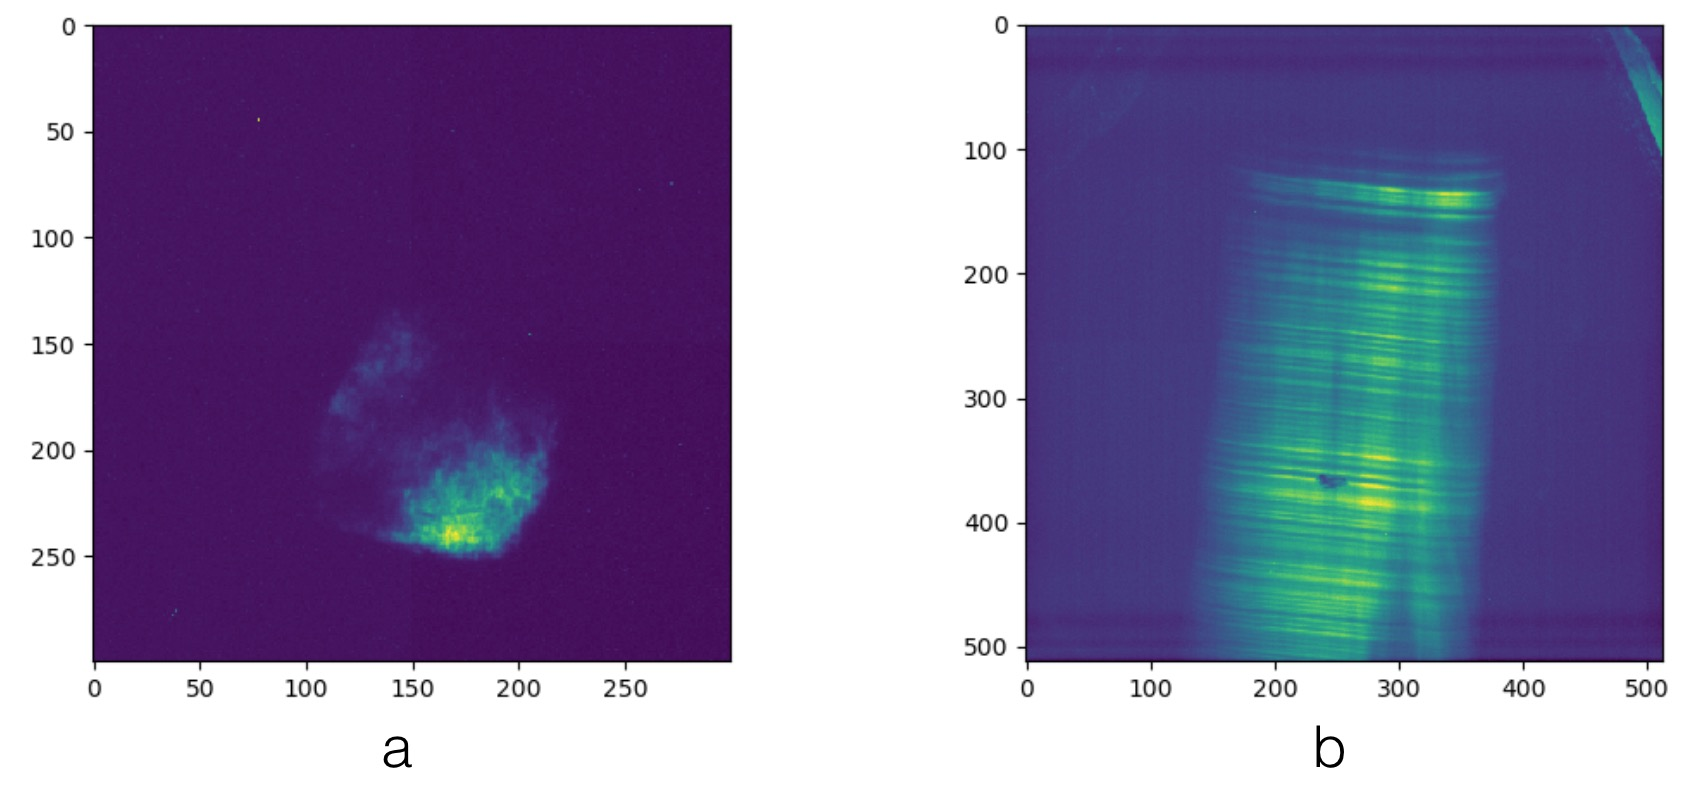
\includegraphics[width=0.75\textwidth]{centered_not_centered}
    \caption{In the current Recon3D version (November 2017), {\texttt{getdata.py}} can only process frames where the diffraction signal is well centered, and it doesn't touch the frame borders, as in {\emph{a}}. The capability to reconstruct samples touching the detector frame ({\emph{b}}) will be later implemented. {\emph{a}} shows a grain in an Al sample (courtesy of Annika Diederichs, {\footnotesize{DTU MEK}}), {\footnotesize{ROI}} size: 300x300; {\emph{b}} shows a crystal in a biomineral sample (courtesy of Phil Cook, {\footnotesize{ESRF}}), {\footnotesize{ROI}} size: 512x512 (entire detector).}
    \label{fig:centered_not_centered}
\end{figure}

\subsection{Roadmap}

The Recon3D manual is structured as follows: at first, the recipe to process the collected data is presented (Sec. {\ref{sec:rec_steps}}), followed by a detailed description of how to run each script (Sec. {\ref{sec:run_scripts}}). Sec. {\ref{sec:data_acquisition}} describes how the experimental data should be collected. In Sec. {\ref{sec:getdata}} and {\ref{sec:recon3d}}, the functioning of {\texttt{getdata.py}} and {\texttt{recon3d.py}} is outlined. In Sec. {\ref{sec:validation}}, the methods used to validate the recon3d reconstruction approach, and provide the final grain reconstruction, are presented.

\subsection{For users - software download}

You can download Recon3D from  \href{https://github.com/albusdemens/Recon3D}{GitHub} and run it on your computer or (highly recommended) on Panda2. Required software: Python and Matlab.

On GitHub, the algorithms to reconstruct the {\footnotesize{3D}} grain shape using the \href{https://github.com/albusdemens/ART-TV-for-DFXRM}{\footnotesize{ART-TV}} and \href{https://github.com/albusdemens/astrarecon}{\footnotesize{ASTRA}} approach are also available.

\subsection{For developers - how to contribute}

Recon3D is an open source project hosted on \href{https://github.com/albusdemens/Recon3D}{GitHub}. To contribute to the code development, clone\footnote{If you don't know what cloning means, check \href{http://product.hubspot.com/blog/git-and-github-tutorial-for-beginners}{this} introduction to Git and GitHub.} the Recon3D distro and have fun!

All code is written in Python, except a few Matlab scripts.

\subsection{Reconstruction steps}
\label{sec:rec_steps}

\subsubsection{Data loading, cleaning and storage}
\label{sec:load_clean_store}

\begin{figure}[h]
    \centering
    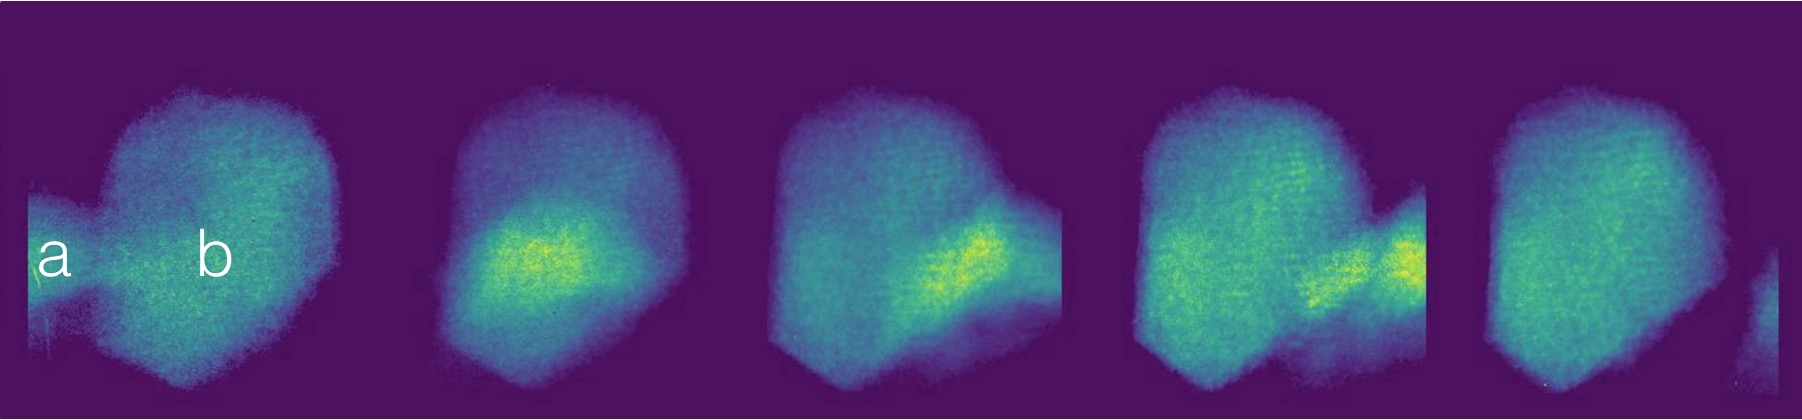
\includegraphics[width=0.9\textwidth]{grain_transit}
    \caption{While investigating grain {\emph{a}}, the transit of grain {\emph{b}} was recorded. This should be avoided.}
    \label{fig:grain_transit}
\end{figure}

\begin{enumerate}
    \item Have a look at the images using \href{https://sourceforge.net/p/fable/wiki/fabian/}{fabian} or {\texttt{plot\textunderscore img.py}}
    \item If necessary, rebin the data using {\texttt{rebin\textunderscore img.py}}: with the current Panda2 configuration, the maximum image size that can be handled is 512$\times$512 pixels (value for 226 projections, 11$\times$11 combinations of $\gamma$ and $\lambda$)
    \item Load the collected images using {\texttt{getdata.py}}, with 0 as threshold value
    \item Visualize the processed images using {\texttt{check\textunderscore threshold.py}}. Look at a few images and select the threshold value to separate the diffraction signal from the background. Afterwards, all intensities below the threshold value will be set to zero
    \item Look at the distribution of the projection angles, returned by {\texttt{getdata.py}}. Is there anything anomalous that should be taken into account? Script: {\texttt{plot\textunderscore angles.py}}
    \item Run {\texttt{getdata.py}}, this time using the threshold value determined in step 4
    \item For each projection, sum up all collected images using {\texttt{img\textunderscore sum.py}}. Save each image sum in a separate file using {\texttt{plot\textunderscore sum.py}}
    \item Load the result as a stack in \href{https://imagej.nih.gov/ij/}{ImageJ} or \href{https://imagej.net/Fiji}{\footnotesize{FIJI}}. {\emph{At present, nor ImageJ nor {\footnotesize{FIJI}} are installed on Panda2. Have a look at the images on your laptop}}
    \item Check how the diffraction projection evolves as the grain rotates. Does the rotation axis move? Are there other grains passing by the detector, as in Fig. \ref{fig:grain_transit}?
    \item If some projection has to be discarded, change the {\texttt{leno}} loops in {\texttt{getdata.py}}, so that only selected projections are loaded. Example: to select projections 1 to 95, 121 to 155 and from 157 to 160, {\texttt{range(leno)}} becomes {\texttt{(range(96) + range(121,156) + range(157, 161))}}. If this is the case, repeat point 5-7
\end{enumerate}

\subsubsection{3D reconstruction}

\begin{enumerate}
    \item Calculate the (possible) rotation axis shift using {\texttt{estimate\textunderscore precession.m}}
    \item Reconstruct the shape of the sample and, for each voxel, determine the orientation by finding the ($\gamma, \mu$) angles for which the maximum intensity was recorded. Code: {\texttt{recon3d.py}}, which among other takes as input the axis rotation shift
    \item Convert the {\footnotesize{3D}} grain shape returned by {\texttt{recon3d.py}} to a {\texttt{vtk}} file, that can be visualized with \href{https://www.paraview.org/}{ParaView}. Script: {\texttt{vol3D\textunderscore vtk.m}}. The script also returns the reconstruction as a {\texttt{.mat}} file
    \item Play with the {\footnotesize{3D}} reconstruction in ParaView
    \item Compare the reconstructed volume with the experimental data using {\texttt{vol3D.m}}. The {\footnotesize{3D}} shape returned by {\texttt{recon3d.py}} heavily depends on the selected {\emph{completeness value}}
\end{enumerate}

\subsubsection{Reconstruction validation and final result}

\begin{enumerate}
    \item The grain shape reconstruction returned by {\texttt{recon3d.py}} greatly depends on which completeness value is chosen. Therefore, it is a good idea to reconstruct the grain shape also using another approach, possibly not dependent on the completeness parameter. Currently, the options available are {\footnotesize{ASTRA}} (GitHub repo: \\ \href{https://github.com/albusdemens/astrarecon}{https://github.com/albusdemens/astrarecon}) and {\footnotesize{ART-TV}} (GitHub repo: \\ \href{https://github.com/albusdemens/ART-TV-for-DFXRM}{https://github.com/albusdemens/ART-TV-for-DFXRM}). At present, the procedure is successfully tested only for the {\footnotesize{ART-TV}} case.

    Steps to validate the recon3d reconstruction and combine it with the one from {\footnotesize{ART-TV}}:
    \begin{enumerate}
        \item Reconstruct the grain shape using {\footnotesize{ART-TV}}. Script: {\texttt{reconstr.m}}, which calls the function {\texttt{ART\textunderscore TV\textunderscore reconstruct\textunderscore 2d\textunderscore new.m}}. As input, the script takes the images summed projection by projection (for the image sum procedure, see point 7 of ``Data loading, cleaning and storage'' \ref{sec:load_clean_store})
        \item Compare the {\footnotesize{3D}} grain reconstruction from {\footnotesize{ART-TV}} with the reconstruction from recon3d and with the experimental data. Script: {\texttt{compare\textunderscore recon3d\textunderscore ART.m}}. The script also combines information from the recon3d reconstruction and from the {\footnotesize{ART-TV}} one in a single volume, with shape defined by the {\footnotesize{ART-TV}} reconstruction. In the selected volume, the voxels have orientation returned by {\texttt{recon3d.py}}
    \end{enumerate}
\end{enumerate}

\subsubsection{ParaView}

ParaView is a software package to visualize and manipulate {\footnotesize{3D}} volumes. A Matlab matrix can easily be saved as a vtk file, that ParaView can read as an input. To load and visualize a volume:

\begin{enumerate}
    \item Click on the eye symbol in the ``Pipeline Browser'' window
    \item Select {\emph{Volume}} as a visualization option
\end{enumerate}

\begin{figure}[h]
    \centering
    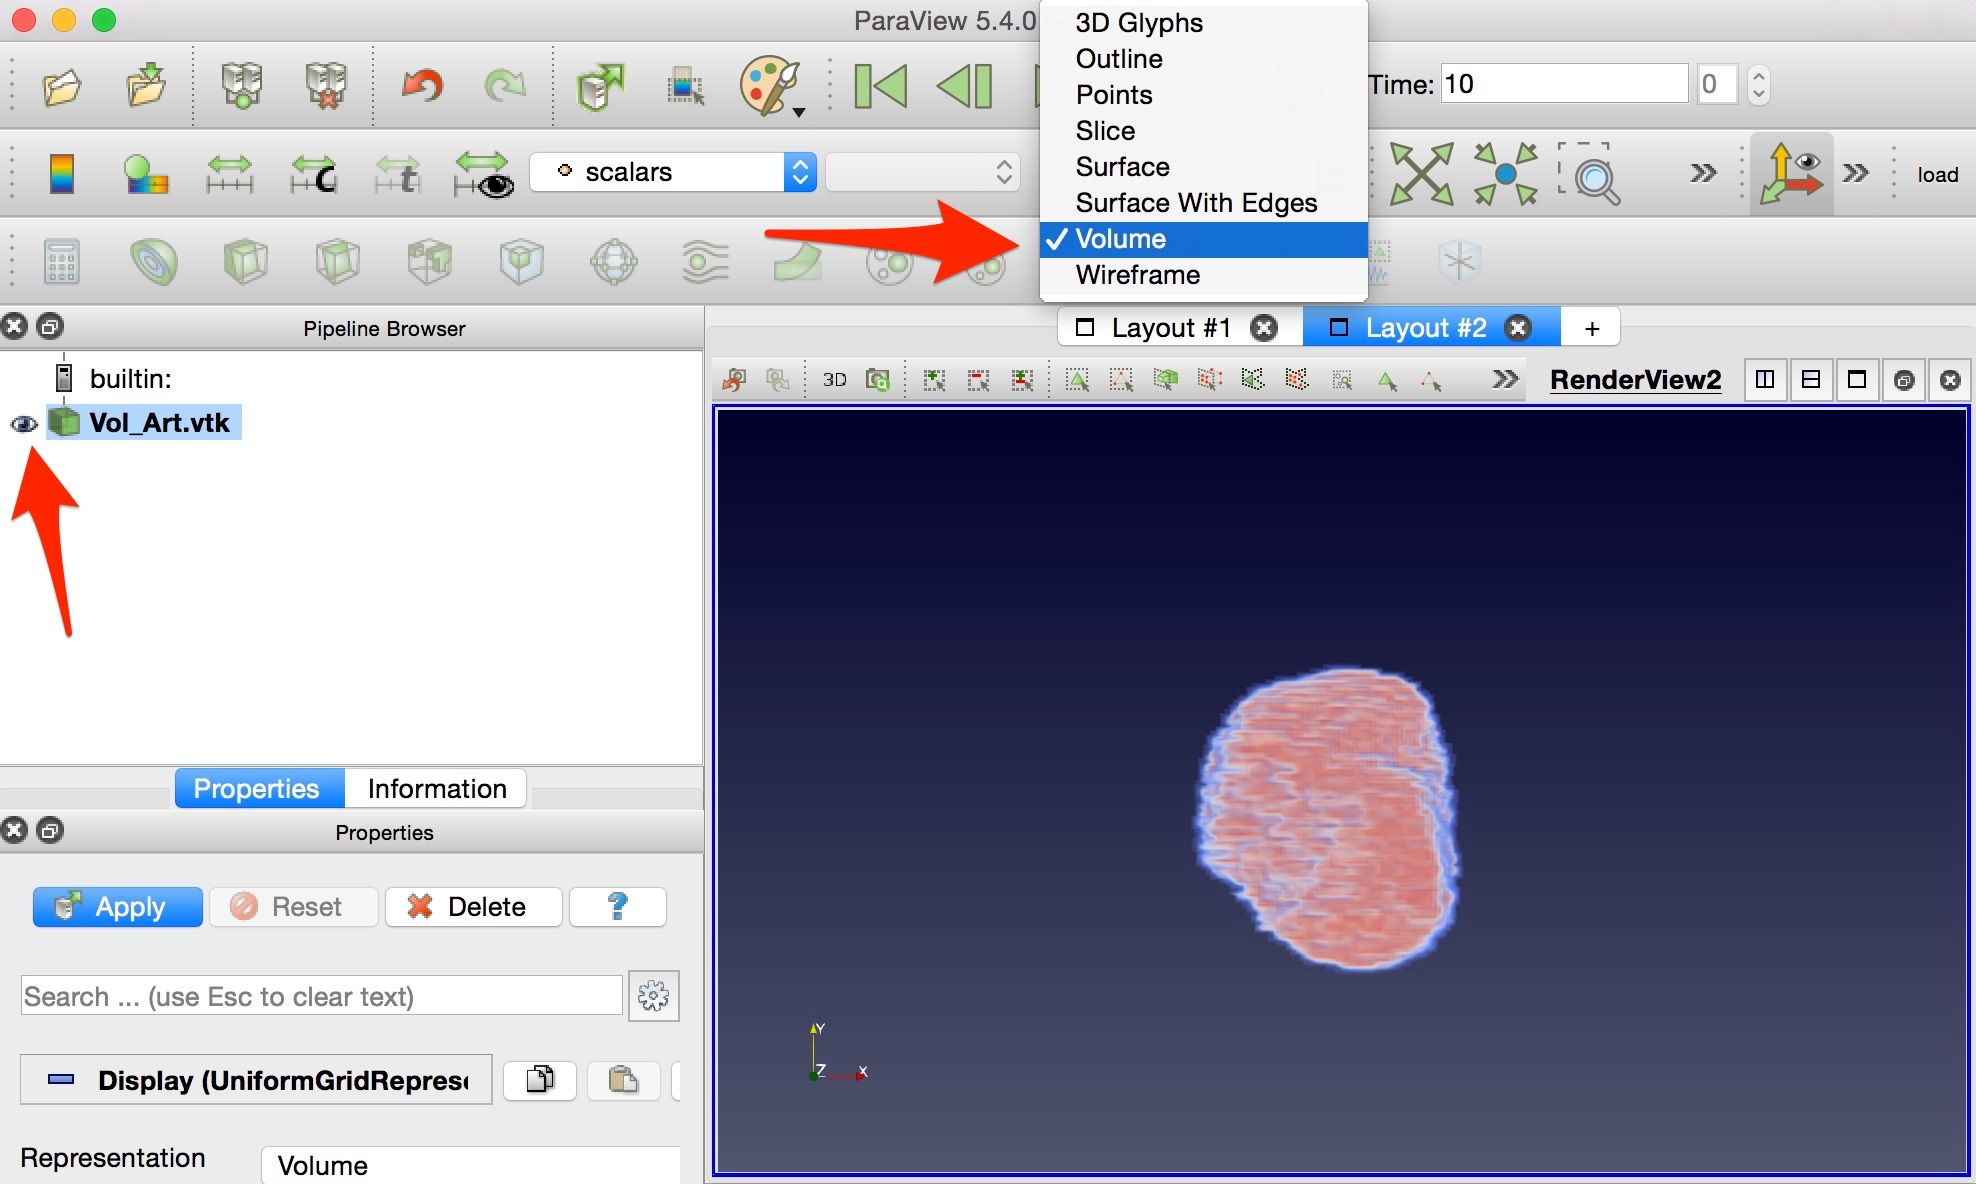
\includegraphics[width=0.75\textwidth]{Paraview_manual.png}
    \caption{ParaView is a user-friendly solution to visualize {\footnotesize{3D}} structures from a {\texttt{vtk}} file. The red arrows indicate how to visualize the data from a vtk file as a {\footnotesize{3D}} object.}
    \label{fig:my_label}
\end{figure}

ParaView can also save animations, with a {\footnotesize{3D}} volume rotating around its axis. To create an animation (see Fig. \ref{fig:PW_animation}),

\begin{itemize}
    \item Select {\texttt{View $\rightarrow$ Animation view}}
    \item In the ``Animation view'' window, add a {\texttt{Camera}} and the {\texttt{vtk}} file you want to animate
    \item Select a reasonable number of frames per second (10 is usually {\footnotesize{OK}})
    \item Hit the play button and enjoy the view
    \item To save the animation, go to {\texttt{File $\rightarrow$ Save animation}}. \danger On {\footnotesize{OSX}}, Quick Time has issues playing the .avi files saved by ParaView. To avoid issues, save the animation as {\texttt{.png}}. This will save separately each single frame, which can then be combined from the command line using \href{http://www.ffmpeg.org/download.html}{\texttt{ffmpeg}}. Check \href{http://hamelot.io/visualization/using-ffmpeg-to-convert-a-set-of-images-into-a-video/}{this} page for the {\texttt{ffmpeg}} syntax. Example: {\texttt{\$ ffmpeg -r 20 -f image2 -s 1248x762 -i Vid.\%04d.png -vcodec libx264 -crf 20 -pix\textunderscore fmt \\ yuv420p Video\textunderscore ART.mov}}
\end{itemize}

\begin{figure}[h]
    \centering
    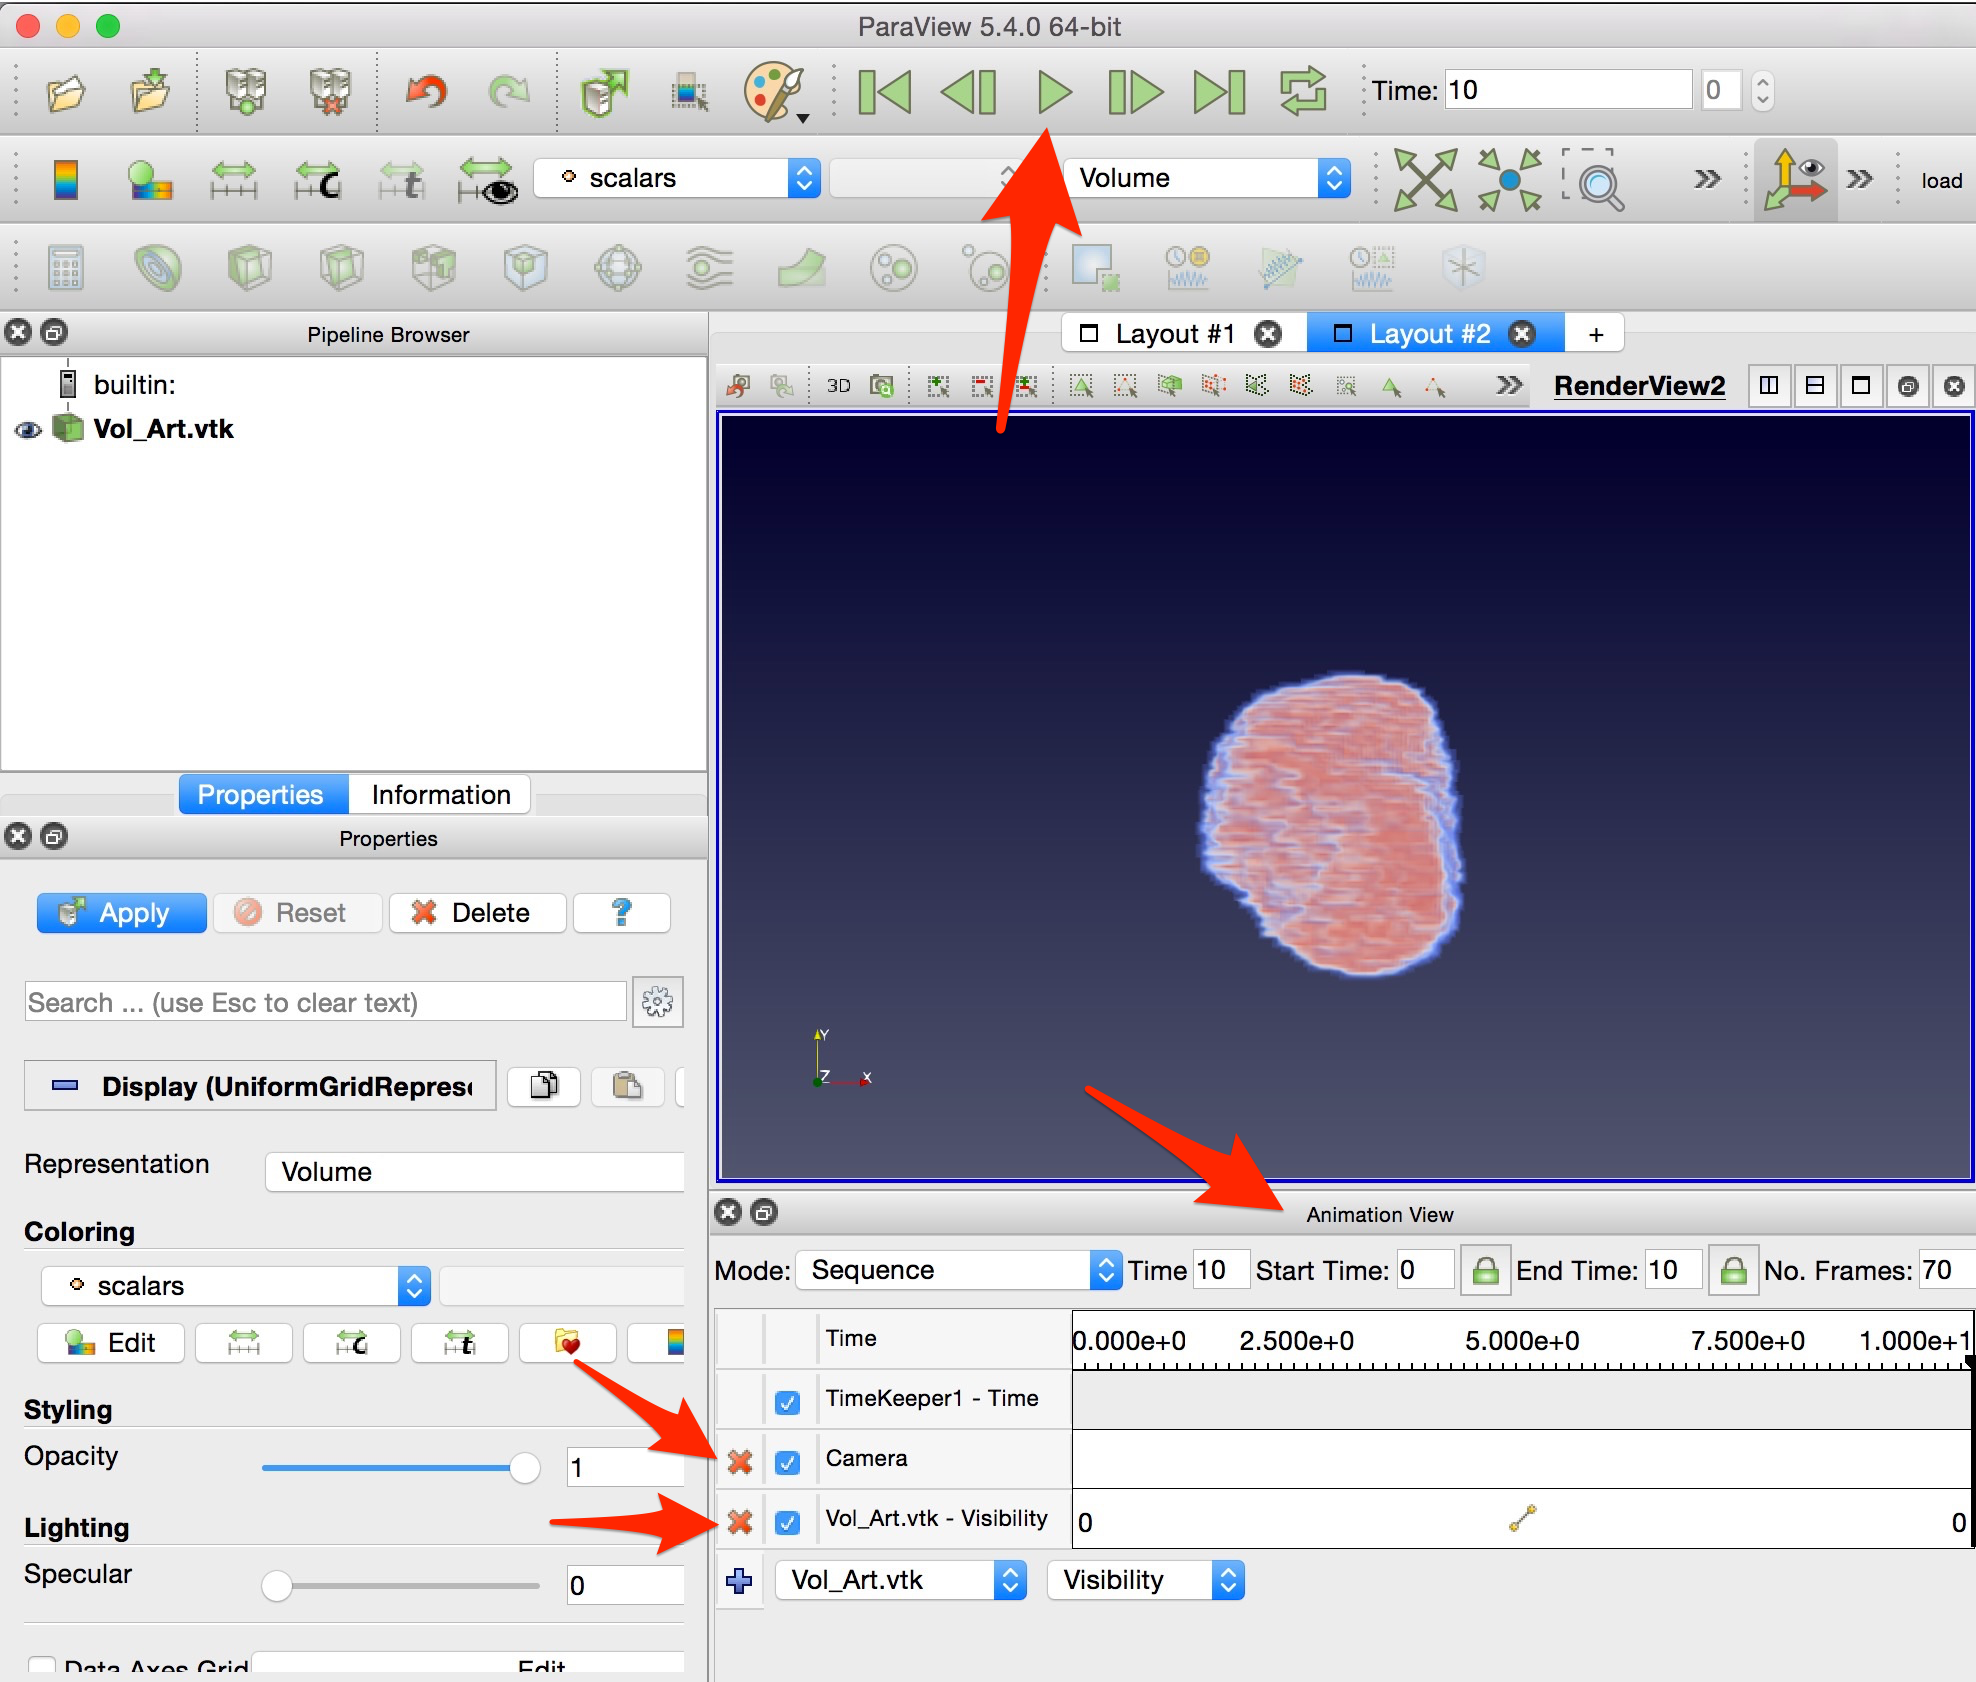
\includegraphics[width=0.75\textwidth]{Animation.png}
    \caption{ParaView can be used to save animations of the reconstructed volumes. Example: grain rotating around a vertical axis.}
    \label{fig:PW_animation}
\end{figure}

\subsection{How to run the Recon3D scripts}
\label{sec:run_scripts}

This section provides an how-to guide to run the scripts to reconstruct the shape and orientation distribution of a grain investigated using {\footnotesize{DFXRM}}.

\subsubsection{A note on mpirun}
\label{sec:mpirun}

When {\texttt{mpirun}} is available (as on Panda2), multiple instances of {\texttt{getdata.py}} and {\texttt{recon3d.py}} can run in parallel, thus increasing the data analysis speed. The maximum number of processes that can run in parallel depends on the available memory. From the terminal, the memory usage can be monitored with the {\texttt{top}} command. If you get a memory error ({\texttt{not enough memory available}} or similar), you should:
\begin{enumerate}
\item Close the current terminal window, or log out from the current ssh session. This will force the memory cleaning
\item If the problem persists, lower the number of {\footnotesize{MPI}} instances
\end{enumerate}

\begin{figure}[h!]
    \centering
    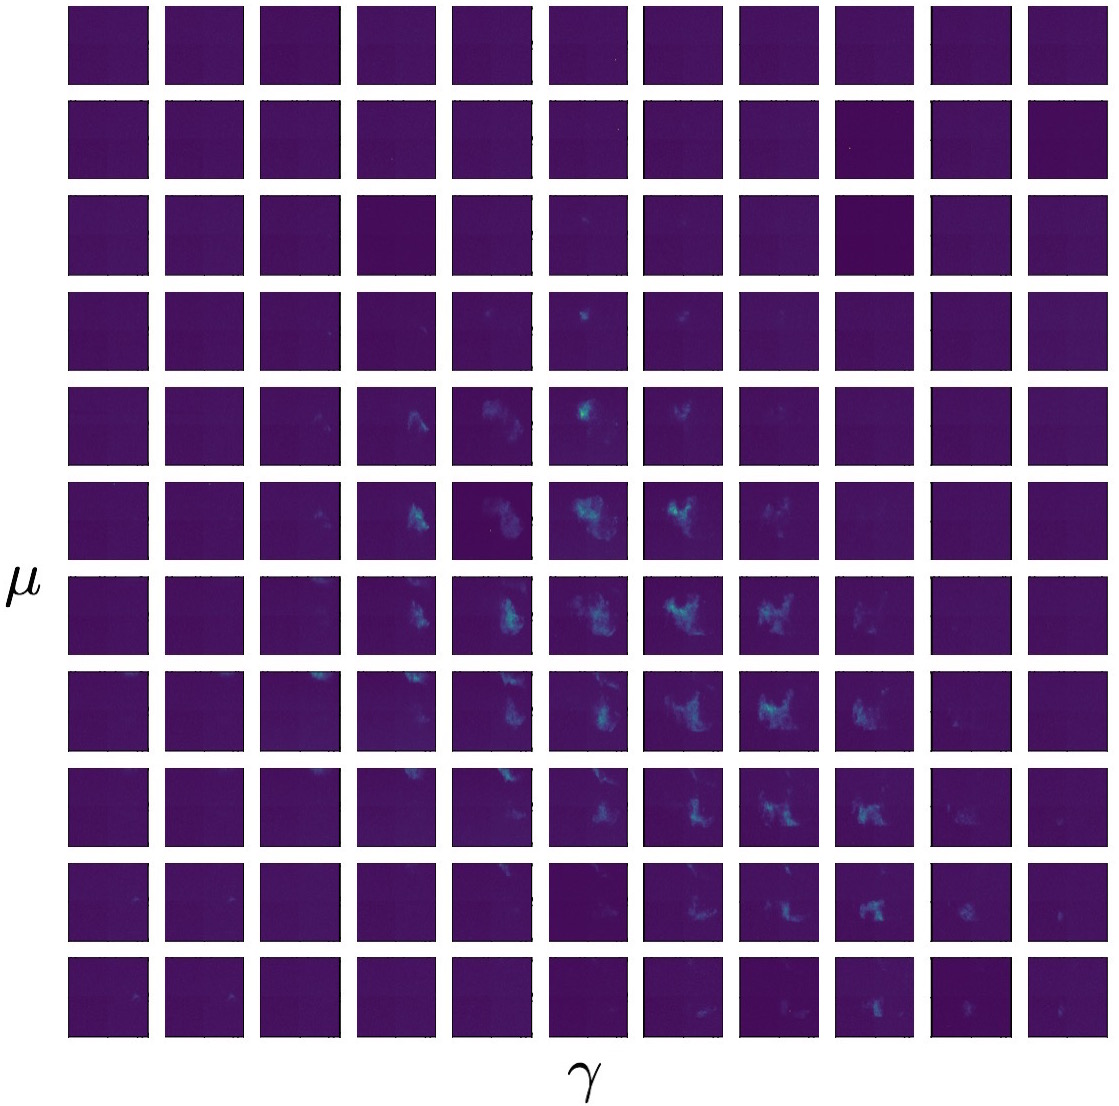
\includegraphics[width=0.85\textwidth]{Img_one_proj}
    \caption{Images collected at a certain rotation angle $\omega$ for different $\gamma$ and $\mu$ angles. For both angles, images were recorded at regular steps with an angular width of 0.0585$^{\circ}$. Sample: deeply embedded grain in a dog-boned Al bar.}
    \label{fig:all_pics_one_om}
\end{figure}

\subsubsection{check\textunderscore threshold.py}

Script to select which threshold value to use to clean the input images with {\texttt{getdata.py}}.

Command:

{\texttt{\$ python check\textunderscore threshold.py [Data directory] [Modality] [Size frame background subtraction] [Number of projections to consider]}}

\begin{itemize}
    \item {\texttt{Data directory}} is the folder where the files returned by {\texttt{getdata.py}} are stored
    \item {\texttt{Modality}}: 1 to show, for each projection, all collected images in an array (like Fig. \ref{fig:all_pics_one_om}); 2 to show, one by one, all images collected at a certain projection
    \item {\texttt{Size frame background subtraction}} is the size of the frame used in {\texttt{getdata.py}} (Sec. \ref{script:getdata}) to clean the frames from a non-isotropic background
    \item {\texttt{Number of projections to consider}} defines how many projections to take into account to determine the threshold value. The projections are selected by dividing the angular range covered during the tomographic scan in the selected number of steps
\end{itemize}

\begin{figure}[h]
    \centering
    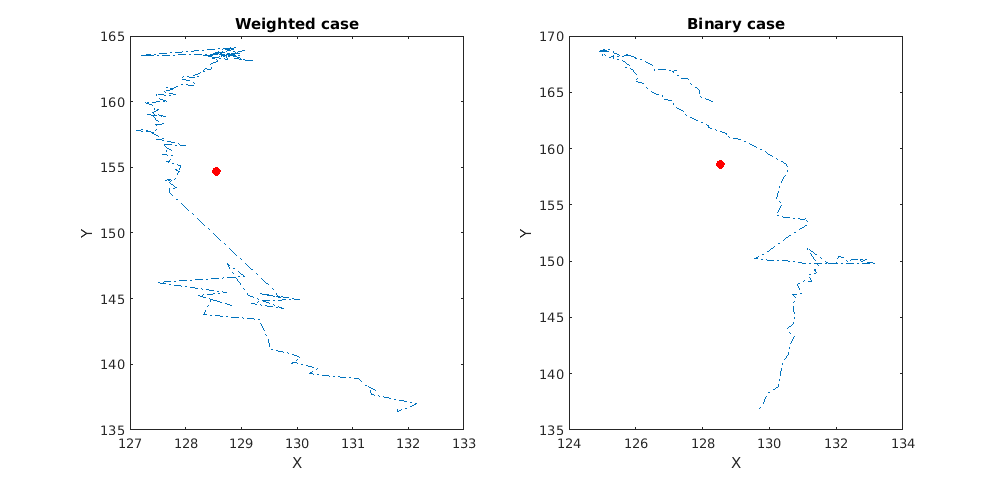
\includegraphics[width=0.8\textwidth]{Estimate_CM.png}
    \caption{Distribution of the center of mass values of the summed diffraction images for an Al grain. {\emph{Left:}} values for the non-binarized image; {\emph{right:}} values for the binarized image. The center of mass of all values is shown as a red dot. Graph generated by {\texttt{estimate\textunderscore precession.m}}.}
    \label{fig:estimate_CM}
\end{figure}

\subsubsection{estimate\textunderscore precession.m}

Script to estimate the position of the sample rotation axis. For each projection, the script calculates the center of mass of the sum of the diffraction signal, returned by {\texttt{img\textunderscore sum.py}}. The center of mass is calculated considering both the image with the sum of the diffraction values and its binarized version (see Fig. \ref{fig:estimate_CM}).

\danger Change input path in the script.

\subsubsection{getdata.py}
\label{script:getdata}

Script to load the {\texttt{.edf}} files (images and header with data), organize the information and return a series of numpy arrays. The functioning of the script is presented in detail in Sec. \ref{sec:getdata}.

Command:

{\texttt{\$ [mpirun -n NN] python getdata.py [Data directory] [Name data files] [Point of interest] [Image size] [Output path] [Output directory] [Initial phi value] [Initial chi value] [Angular step] [Number of angular steps] [Size frame}}

{\texttt{background subtraction] [Image binarization threshold]}}

Inputs:

\begin{itemize}
    \item {\texttt{mpirun -n NN}} allows to run the script using {\texttt{NN}} processors. If {\texttt{mpirun}} is not available, delete this command. For a note on how to use {\texttt{mpirun}}, see Sec. \ref{sec:mpirun}
    \item {\texttt{Data directory}} is the directory storing the {\texttt{edf}} files collected at {\footnotesize{ID06}}
    \item {\texttt{Name data files}} is the file name prefix (without incremental numbers) common to all files
    \item {\texttt{Point of interest}} is the center of the region of interest ({\footnotesize{ROI}}) to be considered
    \item {\texttt{Image size}} is the size of the {\footnotesize{ROI}} to consider. Running the reconstruction code on Panda2, the maximum {\footnotesize{ROI}} size is 512$\times$512. If the frames are bigger, rebin them using {\texttt{Rebin\textunderscore img.py}} (Sec. \ref{sub_s:rebin})
    \item {\texttt{Output path}} is the path to the output directory
    \item {\texttt{Output directory}} is the output directory
    \item {\texttt{Initial phi value}} is the initial value of the $\phi$ motor ($\phi_0$ in Eq. \ref{eq:phi})
    \item {\texttt{Initial chi value}} is the initial value of the $\chi$ motor ($\chi_0$ in Eq. \ref{eq:chi})
    \item {\texttt{Angular step}} is the measure, in degrees, of the interval used to increment $\chi$ and $\phi$ in the data acquisition script
    \item {\texttt{Number of angular steps}} is the number of considered $\chi$ and $\phi$ increments
    \item {\texttt{Size frame background subtraction}} is the size of the cornice used to clean frames from the background signal, to consider possible spatial anisotropies in the detector response. For more details, see Sec. {\ref{subs:data_cleaning}}. {\textit{In a future version of Recon3D, the option to reconstruct grains occupying the entire detector frame (no cornice) will be included}}
    \item {\texttt{Image binarization threshold}} is the threshold value used to select the diffraction spots. All pixels with intensity value below the threshold are set to zero. For more details, see Sec. {\ref{subs:data_cleaning}}
\end{itemize}

Example:

{\texttt{\$ python getdata.py /u/data/andcj/hxrm/Al\textunderscore april\textunderscore 2017/ c6\textunderscore topotomo\textunderscore frelon}}

{\texttt{ \textunderscore far\textunderscore 256,256 300,300 /u/data/alcer/DFXRM test\textunderscore 2 0.69 -1.625 0.0585 11 20}}

{\texttt{12}}

\subsubsection{img\textunderscore sum.py}
\label{sec:img_sum}

Sum, for each projection, all images collected by varying $\gamma$ and $\mu$. Before saving the summed images, have a look at them and select (possible) upper and lower threshold values.

Command:

{\texttt{\$ python img\textunderscore sum.py [Data directory] [Modality] [Lower threshold] [Upper threshold]}}

\begin{itemize}
    \item {\texttt{Data directory}} is the outupt directory of {\texttt{getdata.py}}
    \item {\texttt{Modality}}: 1 to determine threshold values, 2 to check the rotation axis and 3 to prepare the data for {\footnotesize{ASTRA}} and {\footnotesize{ART-TV}}
    \item {\texttt{Lower threshold}} is the lower threshold value. Select 0 for modality 1, modality 2 and if a lower threshold is not necessary
    \item {\texttt{Upper threshold}} is the upper threshold value. Select 0 for modality 1, modality 2 and if an upper threshold is not necessary

\end{itemize}

\subsubsection{plot\textunderscore angles.py}

Shows the distribution of the $\omega$ angles where the sample was scanned.

\subsubsection{plot\textunderscore img.py}

Simple script to plot {\texttt{.edf}} files. To show a file, change path in the code. Alternatively, use the \href{https://sourceforge.net/p/fable/wiki/fabian/}{fabian} module included in FabIO \cite{knudsen2013fabio}

\subsubsection{plot\textunderscore sum.py}
\label{sub_s:plot_sum}

Saves the output from {\texttt{img\textunderscore sum.py}} in {\texttt{png}} files. In this way, the sum of all images collected at a given projection is saved in a different image.

\subsubsection{rebin\textunderscore img.py}
\label{sub_s:rebin}

Script to rebin the collected topotomo frames, to make the dataset manageable by Panda2.

\danger Change paths is the script.

\subsubsection{recon3d.py}

Program to reconstruct the volume of the grain investigated using topotomography.

Command:

{\texttt{\$ [mpirun -n NN] python recon3d.py [Ini file] [Rotation center] [Number acceptable projections]}}

Inputs:

\begin{itemize}
    \item {\texttt{mpirun -n NN}} allows to run the script using {\texttt{NN}} processors. If {\texttt{mpirun}} is not available, delete this command. For a note on how to use {\texttt{mpirun}}, see Sec. \ref{sec:mpirun}
    \item {\texttt{Ini file}} is the file with the crystallographic parameters for the reconstruction. Parameters in the {\texttt{ini file}}:
    \begin{itemize}
        \item {\texttt{sg\textunderscore no}} is the space group number
        \item {\texttt{unit\textunderscore cell}} is the array describing the unit cells parameters ($a,b,c,\alpha, \beta, \gamma$)
        \item {\texttt{wavelength}} is the incoming beam wavelength (in \AA)
        \item {\texttt{grain\textunderscore pos}} is the center of the sample position
        \item {\texttt{grain\textunderscore dim}}, to be calculated using
        \begin{equation}
            {\texttt{grain\textunderscore dim}} = round \Bigg( \frac{{\text{Size {\footnotesize{ROI}}}}}{\texttt{M}} \Bigg)
        \end{equation}
        Where Size {\footnotesize{ROI}} is the size (in pixels) of the {\texttt{edf}} frames considered to reconstruct the sample shape
        \item {\texttt{grain\textunderscore steps}} is the size of the volume (in voxels) containing the sample reconstruction
        \item {\texttt{detx\textunderscore size}} is the {\footnotesize{X}} detector size (in pixels), after binning and before selecting an {\footnotesize{ROI}}
        \item {\texttt{detY\textunderscore size}} is the {\footnotesize{Y}} detector size (in pixels), after binning and before selecting an {\footnotesize{ROI}}
        \item {\texttt{M}} is the magnification value, which depends on the {\footnotesize{CRL}} configuration. The value is measured experimentally
        \item {\texttt{path}} is the location of the {\texttt{getdata.py}} output folder
        \item {\texttt{format}} is the format of the frames collected during the topotomo experiment
        \item {\texttt{mode}} describes the scattering geometry (horizontal or vertical)
    \end{itemize}

    \item {\texttt{Rotation center}} is the estimated {\footnotesize{X}} position of the rotation axis, which can be calculated using {\texttt{Estimate\textunderscore precession.m}}
    \item {\texttt{Number acceptable projections}} is the number of projections with acceptable data (i.e., no information relative to a second grain, \ldots). It is used to calculate, for each voxel, the completeness value
\end{itemize}

Example:

{\texttt{\$ mpirun -n 15 python recon3d.py al\textunderscore test.ini 172 96}}
\subsubsection{vol3D.m}

Script to compare, at different projections, the volume reconstructed by {\texttt{recon3d.py}} with the sum of the recorded diffraction signal.

\danger Change paths in the script.

\subsubsection{vol3D\textunderscore vtk.m}

Script to load the volume reconstructed by {\texttt{recon3d.py}}, select the voxels with completeness greater than 0.5 and save the result as a {\texttt{vtk}} file, which can be visualized in {\footnotesize{3D}} using ParaView.

\subsection{How to run the ART-TV scripts}

The shape of the grain volume reconstructed using the Recon3D approach greatly depends on the choice of the chosen completeness value. To validate the Recon3D reconstruction technique, and obtain a reference {\footnotesize{3D}} reconstruction, the shape of the investigated grain can also be reconstructed using the {\footnotesize{ART-TV}} approach. This section provides an how-to guide to the scripts developed to reconstruct the grain shape using the {\footnotesize{ART-TV}} approach.

\begin{itemize}
    \item {\texttt{reconstr.m}}, which calls {\texttt{ART\textunderscore TV\textunderscore reconstruct\textunderscore 2d\textunderscore new.m}}, is a script to reconstruct the 3D shape of the investigated grain using a combination of {\footnotesize{ART}} and {\footnotesize{TV}}. Input: for each rotation angle, sum of all collected diffraction data (returned by the Recon3D scripts {\texttt{img\textunderscore sum.py}} and {\texttt{plot\textunderscore sum.py}}, Sec. \ref{sec:img_sum} and \ref{sub_s:plot_sum})
    \item {\texttt{Compare\textunderscore recon3d\textunderscore ART.m}}, which
    \begin{itemize}
        \item At selected rotation angles, compares the projections of the {\footnotesize{ART-TV}} and the Recon3D reconstruction with the sum of the collected diffraction data
        \item Combines information from {\footnotesize{ART-TV}} and from Recon3D in a final grain reconstruction, where the grain shape is obtained from the {\footnotesize{ART-TV}} reconstruction approach, and each voxel has orientation calculated by Recon3D
    \end{itemize}
\end{itemize}

\section{Recommendation for data acquisition}\label{sec:data_acquisition}

\subsection{Data acquisition script}

{\texttt{getdata.py}} is designed to treat data acquired using a macro script structured as follows:

\begin{lstlisting}
def topotomoscan '{

    getinitpos

    _omegastart = 0
    _omegaend = 180
    _omegastepsize = 0.8
    _omegasteps = (_omegaend-_omegastart)/_omegastepsize

    for(_omegai = 0; _omegai <= _omegasteps; _omegai += 1){

        _omega = _omegastart + _omegai*_omegastepsize
        printf("\n OMEGA = %g\n", _omega)
        umv diffry _omega

        _phistepsize = cos(rad(_omega))*0.032
        _chistepsize = sin(rad(_omega))/cos(rad(_zpchi))*0.032
        for(_secondi = 0; _secondi <= 6; _secondi += 1){
            _phi = _zpphi + (_secondi-3)*_phistepsize
            _chi = _zpchi + (_secondi-3)*_chistepsize
            printf("\n chi = %g, phi = %g\n", _chi, _phi)
            umv chi _chi phi _phi

            zapline diffrz _zpdiffrz-3.5*0.032 _zpdiffrz+3.5*0.032 7 2000
        }

    }


    movetoinit

}'
\end{lstlisting}

In particular, it is important that {\texttt{\textunderscore chistepsize}} and {\texttt{\textunderscore phistepsize}} are described as above (lines 16 and 17). If data have been acquired in the opposite way

\begin{lstlisting}
        _phistepsize = sin(rad(_omega))/cos(rad(_zpphi))*0.032
        _chistepsize = cos(rad(_omega))*0.032
\end{lstlisting}

In {\texttt{getdata.py}}, function {\texttt{calcGamma(self, data)}}, substitute {\texttt{self.meta[ind,0]}} with \\ {\texttt{self.meta[ind,1]}}, and {\texttt{data.alpha0}} with {\texttt{data.beta0}}.

\section{getdata.py}
\label{sec:getdata}

\begin{figure}[h]
    \centering
    \label{fig:img_array}
    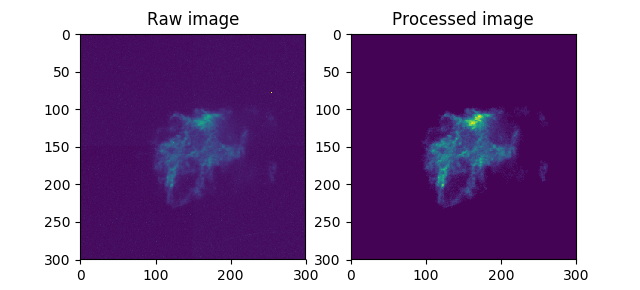
\includegraphics[width=0.9\textwidth]{Raw_processed}
    \caption{Outline of the data processing procedure included in {\texttt{getdata.py}}. {\emph{Left:}} typical {\footnotesize{DFXRM}} raw image; {\emph{right:}} image after the data processing procedure included in {\texttt{getdata.py}}.}
    \label{fig:raw_processed}
\end{figure}

{\texttt{getdata.py}} is a script to load, process and store the {\texttt{.edf}} files collected during a topotomo scan. The goal of the data processing steps is to minimize the noise contribution, enhance the signal from the diffraction spot and normalize the intensity values from different projections.

\subsection{Input data}

Fig. \ref{fig:all_pics_one_om} shows the frames recorded, at a given projection, by varying $\gamma$ and $\mu$ by a constant angular increment ({\emph{topotomo scan}}). The shape of the recorded diffraction spot noticeably changes among frames. This agrees with what expected: for different combinations of $\gamma$ and $\mu$, the Bragg condition is satisfied by different substructures of the considered grain.

As input, {\texttt{getdata.py}} loads a set of frames collected during a topotomo scan. The frames are saved as {\texttt{edf}} files, each consisting of the actual detector image and of a header storing the parameters at which each frame has been collected (e.g. motor position, ring current, \ldots) For each {\texttt{edf}} file , {\texttt{getdata.py}} stores the key information from the header, and the actual image, in a five-dimensional matrix: two dimensions are used to store the image, and the other three to keep record of the combination of angles at which the image has been recorded. The angles are:
\begin{itemize}
    \item $\omega$, the sample rotation angle
    \item $\mu$, the in-plane sample tilting angle
    \item $\gamma$, the off-plane sample tilting angle perpendicular to $\mu$. The value of $\gamma$ is determined by a {\emph{pseudomotor}}, which is not a real motor but instead a combination of the motors controlling the angles $\chi$ and $\phi$ (a.k.a. $\alpha$ and $\beta$), regulated so that $\gamma$ and $\mu$ always move on two perpendicular planes. In the data acquisition script in Sec. \ref{sec:data_acquisition}, $\chi$ and $\phi$ are defined as

    \begin{eqnarray}
        \chi & = & \chi_0 + i \cdot \Delta \chi \label{eq:chi} \\
             & = & \chi_0 + i \cdot \frac{\sin\omega}{\cos\phi_0} \cdot \Delta\chi \\
        \phi & = & \phi_0 + i \cdot \Delta \phi \label{eq:phi} \\
             & = & \phi_0 + i \cdot \cos\omega \cdot \Delta\phi
    \end{eqnarray}

    Where $\phi_0$ and $\chi_0$ are the initial positions of the $\phi$ and $\chi$ motors, and $\Delta\phi$ $[\Delta\chi]$ is the angular step used to increment the $\phi$ $[\chi]$ position. Denoting the increment of the pseudomotor position with $\Delta\gamma$, with $\Delta\gamma = \Delta\phi = \Delta\chi$, from Eq. \ref{eq:phi} $\gamma$ can be calculated as

    \begin{equation}
        \gamma = i \Delta\gamma = \frac{\phi - \phi_0}{\cos\omega}
    \end{equation}

    To read the header of the {\texttt{.edf}} images, modules from the FabIO\cite{knudsen2013fabio} package were used.

\end{itemize}

\subsection{Output}

{\texttt{getdata.py}} generates the following output files:

\begin{itemize}
    \item {\texttt{mu.npy}} - a file listing the considered scattering angles where frames where collected. Values read from the header of the {\texttt{.edf}} files
    \item {\texttt{gamma.npy}} - a file listing the values of $\gamma$, a pseudoangle (it's a combination of $\chi$ and $\phi$, and it's not controlled by a real motor) perpendicular to $\mu$. The $\chi$ and $\phi$ values are read from the header of the {\texttt{.edf}} files
    \item {\texttt{omega.npy}} - a file listing the considered sample rotation angles (in degrees). Values read from the header of the {\texttt{.edf}} files
    \item {\texttt{dataarray.npy}} - a file storing, as a five-dimensional matrix, the coordinates of each diffracted intensity value collected during a topotomo scan. The dimensions are: $\gamma$ angle, $\mu$ angle, $\omega$ angle, X coordinate, Y coordinate. In other words, {\texttt{dataarray.npy}} stores the raw images as a function of the angles where they were collected
    \item {\texttt{cleaning\textunderscore img.npy}} - a file containing, for each considered projection, the frame used to correct frames for the background current. Dimensions: $\omega$ angle, {\footnotesize{X}} coordinate, {\footnotesize{Y}} coordinate
    \item {\texttt{dataarray\textunderscore clean.npy}} - a file structured as {\texttt{dataarray.npy}}, contains the collected frames after they have been normalized by the mean, so that the total integrated intensity is the same for each projection
    \item {\texttt{dataarray\textunderscore final.npy}} - a file structured as {\texttt{dataarray.npy}}, which contains the frames after the preprocessing procedure
    \item {\texttt{Image\textunderscore properties.txt}} - a text file listing the number of each image and the $\gamma$, $\mu$ and $\omega$ angle where it was collected. $\gamma$, $\mu$ and $\omega$ are read from the header of the {\texttt{.edf}} files
\end{itemize}

\subsection{Data cleaning}
\label{subs:data_cleaning}

Nomenclature: a {\emph{projection}} is a sample rotation angle $\omega_i$ where data was acquired; a {\emph{frame}} is a detector image collected at a certain set of $(\gamma, \mu, \omega)$ angles.

\begin{figure}[h]
    \centering
    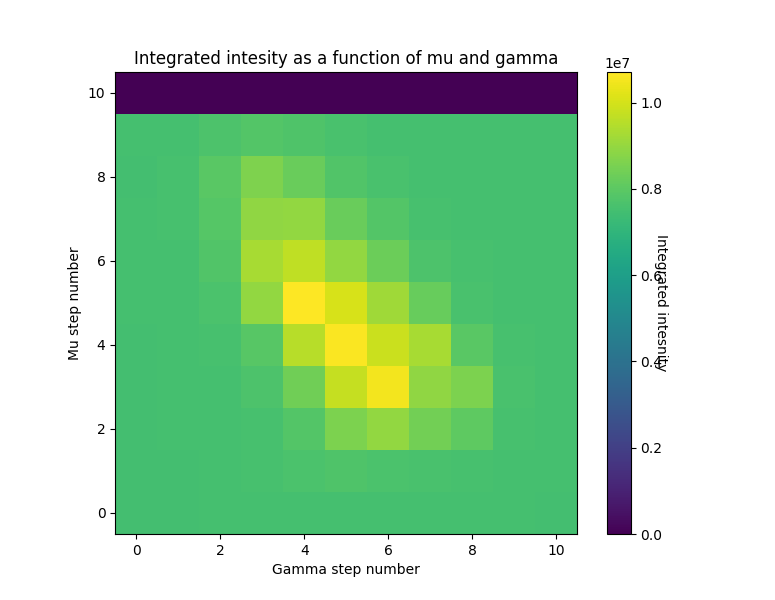
\includegraphics[width=0.62\textwidth]{Distr_I_int}
    \caption{Distribution of the integrated intensity for the frames recorded at a certain projection $\omega_i$ by varying $\gamma$ and $\mu$. Each pixel represents a different frame. For both $\gamma$ and $\mu$, the step size is 0.0585$^{\circ}$. For a given projection, the first step to clean the recorded frames is to subtract, pixel by pixel, from each frame the average of the two images, collected at the same projection, with the lower integrated intensity.}
    \label{fig:distr_I_int}
\end{figure}

These are the steps followed to clean the collected frames:
\begin{enumerate}
    \item For a given projection, subtract from each frame the dark current (detector readout when there is no incoming signal). The dark current frame is estimated as follows (lines 170-211 in {\texttt{getdata.py}}):
    \begin{enumerate}
        \item Calculate the integrated intensity of each frame (see Fig. \ref{fig:distr_I_int})

        \item Select the two frames with the lower (but greater than 0) integrated intensities: $I_{min,1}$ and $I_{min,2}$. If there aren't at least two images with nonzero integrated intensity, define the dark current frame as made of zeros

        \item Calculate,pixel by pixel, the average value of $I_{min,1}$ and $I_{min,2}$:
        \begin{equation}
            <I_{min}(x,y)> = \frac{I_{min,1}(x,y) + I_{min,2}(x,y)}{2}
        \end{equation}
        Where the pixel by pixel operation takes into account possible spatial anisotropies

        \item Subtract from each frame the dark current frame, $<I_{min}(x,y)>$

        \item Set negative pixels to 0

        \item Threshold the hot pixels
    \end{enumerate}

    \item Normalize the recorded frames by requiring that the total integrated intensity (sum of the images collected varying $\gamma$ and $\mu$) is the same for each projection. In this way, we take into account possible
    variations of the beam power during the experiment. For a given projection, the steps are (lines 217-230 in {\texttt{getdata.py}}):
    \begin{enumerate}
        \item Sum all recorded frames

        \item Calculate the mean pixel intensity

        \item Normalize, pixel by pixel, each frame by dividing by the mean intensity of the relative projection, and multiplying by the mean of all the mean intensity values, each relative to a different projection (see Fig. \ref{fig:I_normalization})
            \begin{equation}
                I_{normalized}(x,y)_{\gamma, \mu, \omega} = \frac{I(x,y)_{\gamma, \mu, \omega}}{<\sum_{\gamma, \mu} (x,y)>_{\omega}}\cdot <<\sum_{\gamma, \mu} (x,y)>_{\omega}>
            \end{equation}
    \end{enumerate}

    If there are projections where no intensity is recorded, they should be excluded from the calculation of the mean values.
    \begin{figure}[h]
    \centering
    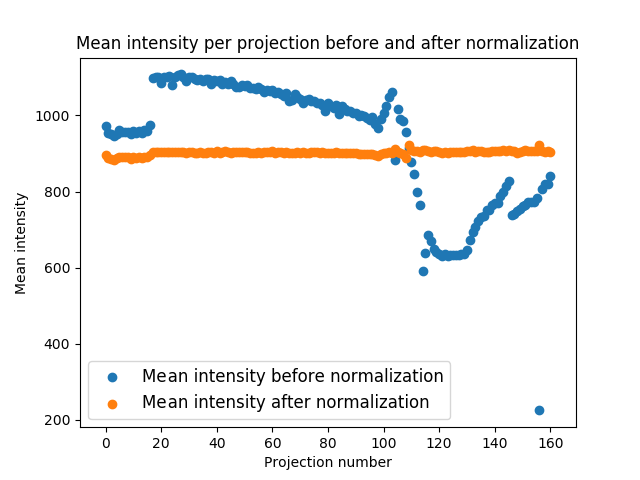
\includegraphics[width=0.75\textwidth]{I_before_after_normalization}
    \caption{Mean pixel intensity per projection before and after the normalization process included in {\texttt{getdata.py}} (Sec. \ref{subs:data_cleaning}).}
    \label{fig:I_normalization}
    \end{figure}

    \item For each frame collected at a given projection, characterize the noise distribution and subtract it from the recorded intensity (lines 233-273 in {\texttt{getdata.py}}). Goal: minimize the noise and consider possible spatial anisotropies of the detector response.

    \danger {\emph{Wolfgang Ludwig from {\footnotesize{ESRF}} suggested that this should not be necessary if the transfocator is managed correctly}}.

    For every image collected at a given projection the steps are, as illustrated in Fig. \ref{fig:binning}:
    \begin{enumerate}
        \item Rebin the image (the size of the bins corresponds to the {\texttt{Size frame background subtraction}} given as an input to {\texttt{getdata.py}})

        \begin{figure}[h]
        \centering
        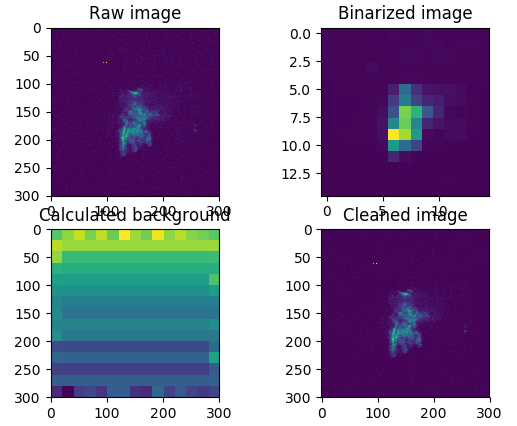
\includegraphics[width=0.75\textwidth]{Background_characterization}
        \caption{Steps followed to clean each image from its background signal. At first, the collected frames are binned (bin size provided as {\texttt{Size frame background subtraction}} to {\texttt{getdata.py}}). The outermost bins, where no diffraction signal is expected, are used to calculate the expected background distribution for the entire image. The background is then subtracted from the image.}
        \label{fig:binning}
        \end{figure}

        \item Consider the cornice of the rebinned image (first and last column, first and last row), where normally there is no diffraction signal.

        \danger {\emph{This should be changed in case of bad alignment}}

        \item Notice that the background signal tends to progressively increase/decrease along Y

        \item Calculate, for each pixel, the expected background signal using the intensity values of the top and bottom bin from the same column. For a pixel with coordinates $(x,y)$, $IB_{bin,min}$ and $IB_{bin, max}$ are the maximum and minimum background signal intensities, calculated considering the top and bottom bins corresponding to the $x$ column. The intensity of the background signal in a pixel located in $(x,y)$, $IB(x,y)$, is then
        \begin{equation}
            IB(x,y) = IB_{bin,min} + \frac{IB_{bin,max} - IB_{bin,min}}{sz(image) - 2\cdot sz(cornice)}\cdot(y - sz(cornice))
        \end{equation}
        Where $sz(frame)$ and $sz(cornice)$ are the size of the image (before binning) and of the cornice, respectively

        \item Subtract the calculated background from the frame

        \item Set all negative pixels to zero
    \end{enumerate}

    \begin{figure}[h!]
        \centering
        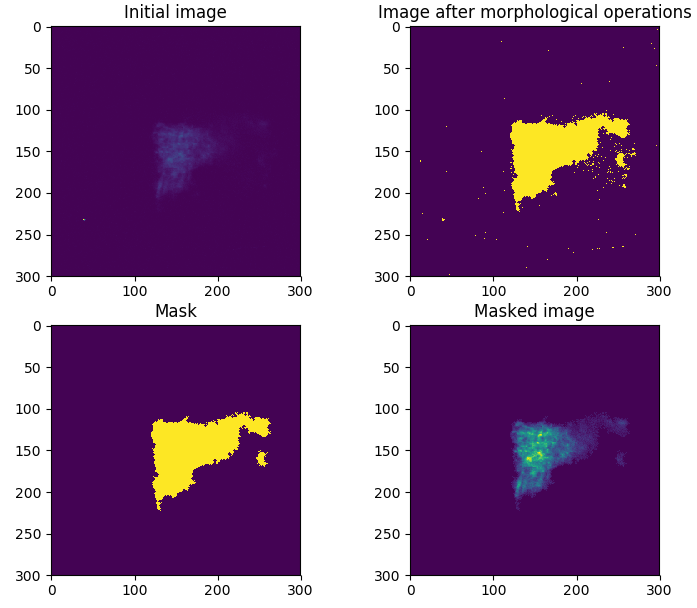
\includegraphics[width=0.75\textwidth]{Morph_ops}
        \caption{The final step of the developed image processing procedure consists in localizing the diffraction spots, and setting to 0 all pixels that are not part of them. This is done by binarizing the image, performing morphological operations, selecting the larger regions and making a mask using them.}
        \label{fig:morph_ops}
    \end{figure}

    This procedure can only be performed if the collected diffraction spots always occupy a region that is well centered on the detector surface. If that is not the case, set the cornice size to 0.

    \item Localize the regions containing the diffraction signal and set to 0 all pixels outside it (see Fig. \ref{fig:morph_ops}). Lines 272-294 in {\texttt{getdata.py}}. In detail, the steps are:
    \begin{enumerate}
        \item Threshold the input image (threshold value provided as input to {\texttt{getdata.py}}) and binarize the result

        \item Fill the holes in the image, and perform the morphological operations of erosion and dilation \cite{image_book}. In Python, a fast and easy way to do so is to use the functions included in \href{http://scikit-image.org/}{skimage} and \href{https://docs.scipy.org/doc/scipy/reference/tutorial/ndimage.html}{ndimage}. Code snippet from {\texttt{getdata.py}}:
        \begin{verbatim}
from skimage.morphology import disk, dilation, erosion
Cleared = ndimage.binary_fill_holes(IM_clean_bin).astype(int)
Dilated = erosion(dilation(Cleared, disk(1)), disk(1))
Dilated_c = ndimage.binary_fill_holes(Dilated).astype(int)
        \end{verbatim}

        \item Label the regions in the resulting binary image, and select only those with an area larger than 100 pixels.

        \danger {\emph{The minimum number of pixels required to consider a cluster as a diffraction spot depends on the noise and the signal distribution for a specific sample. A reasonable value should be determined through tests}}

        \item Using the selected regions, mask the initial image and set all pixels outside the mask to 0
    \end{enumerate}

\end{enumerate}

%{\texttt{getdata.py}} also returns an array containing, for each projection, the sum of all collected images. The summed images have been normalized so that they have the same summed intensity. For a given projection {\emph{i}}, the summed image was normalized pixel by pixel using the formula

%\begin{equation}
%    I_{i,normalized}(x,y) = \frac{I_i(x,y)}{mean(I_i(x,y))} \cdot max\{mean(I_i(x,y))\}_i
%\end{equation}

\section{recon3d.py}
\label{sec:recon3d}

The {\texttt{recon3d.py}} script reconstructs the {\footnotesize{3D}} shape and the orientation distribution of a single, deeply embedded grain from a topotomo dataset collected at {\footnotesize{ID06}}.

The script uses a forward model, which for a given voxel calculates the position of the corresponding diffraction spots on the detector surface as a function of $\omega, \gamma$ and $\mu$. For each voxel, the diffracted intensity values collected at different ($\omega, \gamma, \mu$) values are stored. The $\gamma, \mu$ combination that consistently gives the higher intensity is selected as the orientation of the voxel. The quality of the reconstruction increases with the number of available projections (see Fig. \ref{fig:recon3d_different_ranges}).

\begin{figure}[h]
    \centering
    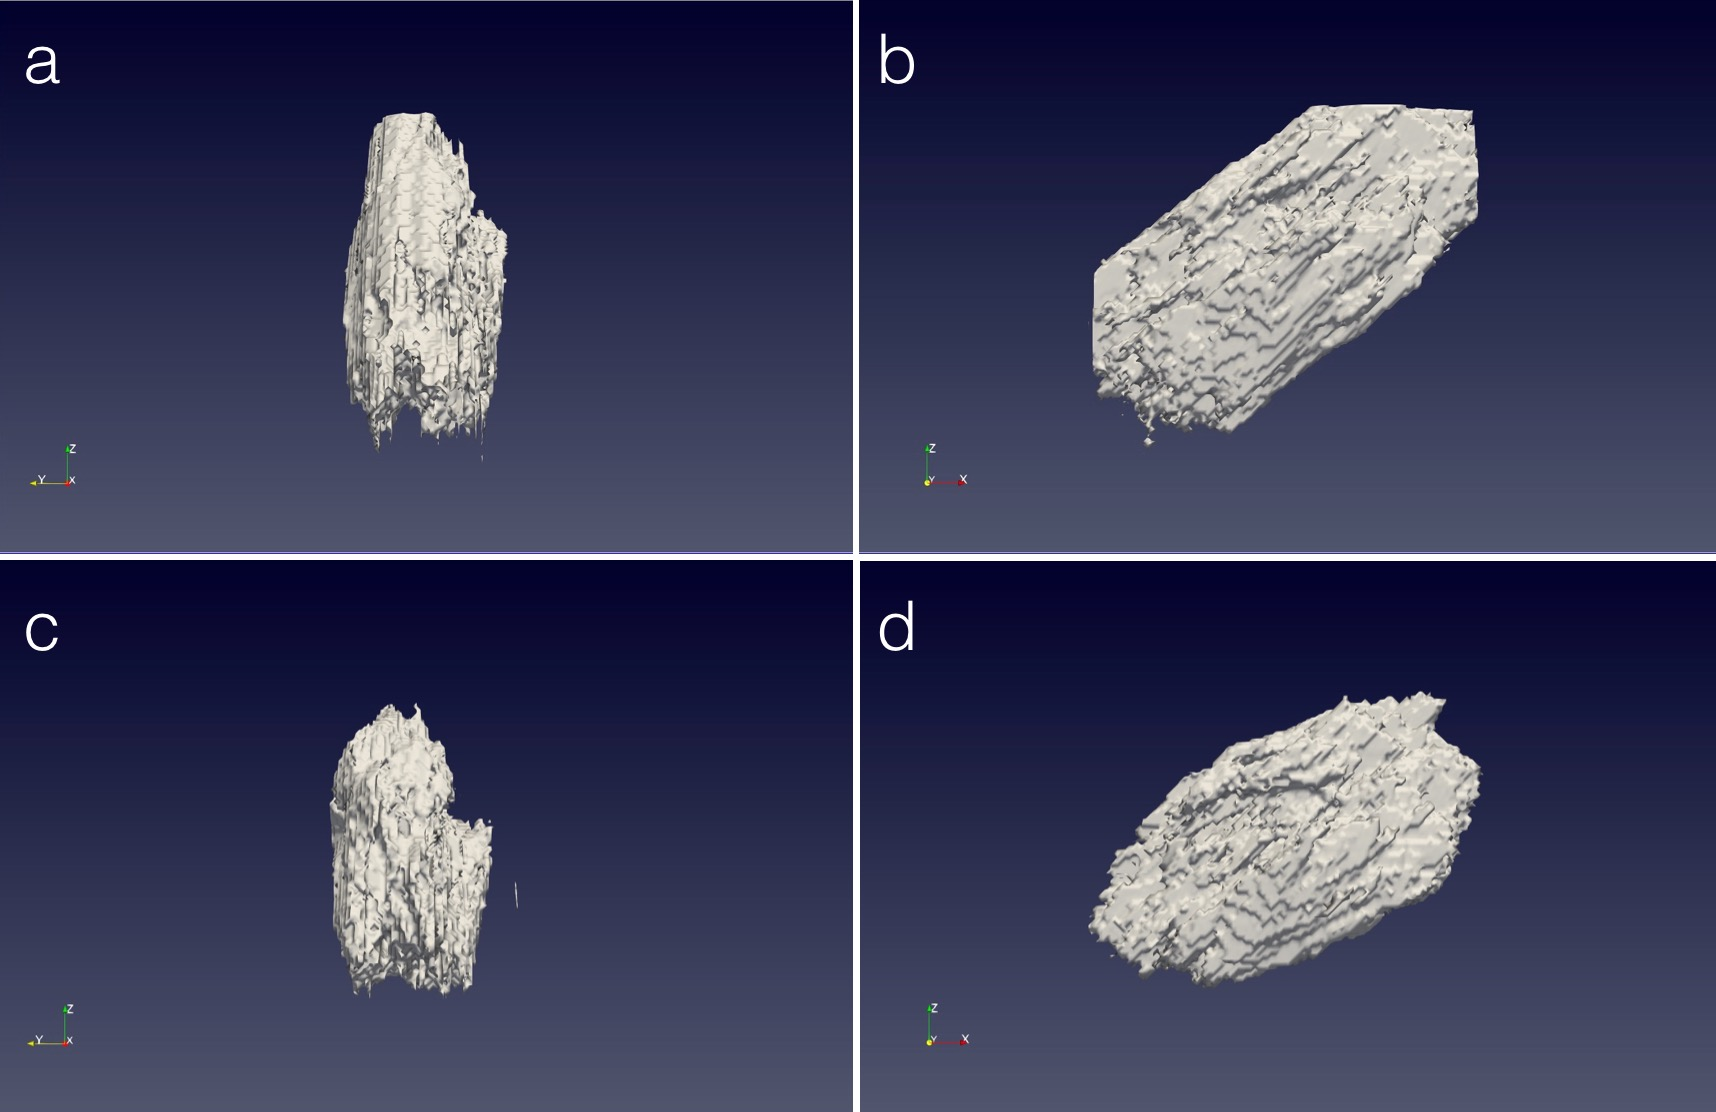
\includegraphics[width=0.9\textwidth]{recon3d_different_ranges.png}
    \caption{The quality of the recon3d sample reconstruction increases with the number of available projections. {\emph{a}} and {\emph{b}}: projections of the reconstruction obtained using 96 projections, 0.8$^{\circ}$ step, 76.8$^{\circ}$ coverage. {\emph{c}} and {\emph{d}}: projections of the reconstruction obtained adding to the 76.8$^{\circ}$ coverage another 60.8$^{\circ}$, sampled in 1.6$^{\circ}$ steps.}
    \label{fig:recon3d_different_ranges}
\end{figure}

In other words, {\texttt{recon3d.py}} consists of a set of transformation from the sample reference system to the detector reference system. The approach is presented in detail in the white paper \cite{report_jette_anders}. For consistency with the current definition of the geometry \cite{henning_joac}, the rolling angle is denoted with $\chi$ (in the white paper it's $\phi_{up}$) and the rocking angle is denoted with $\phi$ (in the white paper it's $\phi_{lo}$).

\begin{table}[h]
    \begin{center}
    \begin{tabular}{ c c c }
        Notation {\footnotesize{JOAC}} & Notation {\footnotesize{HFP}} & Meaning \\
        $\phi_{up}$ & $\chi$ & Rolling \\
        $\phi_{lo}$ & $\phi$ & Rocking \\
    \end{tabular}
    \end{center}
    \caption{To study the orientation distribution inside the {\footnotesize{3D}} volume of a grain, for each projection the sample is rolled and rocked. {\footnotesize{JOAC}} is the notation used in \cite{report_jette_anders}, and {\footnotesize{HFP}} is the ``new'' notation \cite{henning_joac}.}
    \label{tab:angles}
\end{table}

\subsection{Code structure}

Designed to optimize speed, {\texttt{recon3d.py}} is structured as follows:
\begin{enumerate}
    \item Definition of the matrices describing the transformation from the sample reference system to the detector reference system
    \item Calculation of the transformation matrix for all possible combinations of ($\omega, \gamma, \mu$). Store the calculated matrices
    \item For a given voxel, consult the calculated matrices and find the position of the corresponding detector pixel as a function of ($\omega, \gamma, \mu$)
    \item For a given voxel, store each ($\omega, \gamma, \mu$) combination and the intensity value of the corresponding detector pixel (calculated in the previous step)
\end{enumerate}

\subsection{Definition of a voxel orientation}

With {\footnotesize{DFXRM}}, the orientation of a voxel is defined by a ($\mu, \gamma$) combination. This is determined by (see Fig. \ref{fig:mosaicity_map}).
\begin{enumerate}
    \item Summing in a unique map all the maps showing, for each $\omega$, the ($\gamma, \mu$) combinations of the pixels relative to the selected voxel
    \item Selecting the maximum of the summed map as the ($\gamma, \mu$) orientation of the selected voxel
\end{enumerate}

\begin{figure}[h]
    \centering
    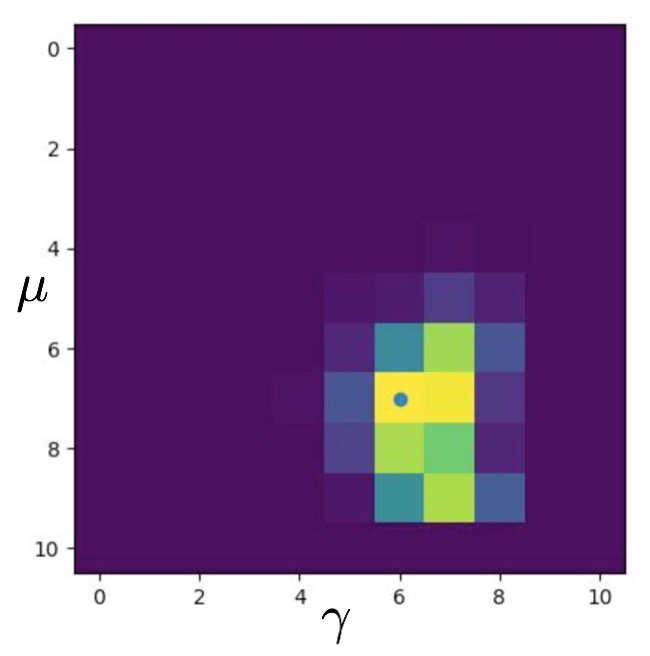
\includegraphics[width=0.5\textwidth]{Mosaicity_map.png}
    \caption{Sum of the ($\gamma, \mu$) values relative to a voxel. The position of the maximum value, selected as voxel orientation, is indicated with a red spot.}
    \label{fig:mosaicity_map}
\end{figure}

To evaluate the accuracy of the orientation determination, the {\emph{completeness}} $C$ is considered, defined as

\begin{equation}
    C = \frac{\text{Number of projections where the } (\gamma, \mu) \text{ orientation is measured}}{\text{Number of considered projections}}
\end{equation}

\section{Validation of the shape reconstruction procedure}
\label{sec:validation}

The {\footnotesize{3D}} grain shapes reconstructed by Recon3D greatly depend on the choice of the completeness value {\emph{C}}. To cross-check the validity of the Recon3D reconstruction two other reconstruction methodologies are available, based on the {\footnotesize{ASTRA}} Toolbox \cite{van2015astra, van2016fast} and on {\footnotesize{ART-TV}} \cite{laroque2008accurate}, which is a combination of the Algebraic Reconstruction Technique ({\footnotesize{ART}}) with the Total Variation ({\footnotesize{TV}}) approach. As input, both methodologies take one image per projection, obtained by summing all frames collected while varying $\mu$ and $\gamma$.

In the following, the geometry and the reconstruction scripts of both methodologies are presented.

\subsection{Validation using ASTRA}

The {\footnotesize{ASTRA}} toolbox \cite{van2015astra, van2016fast} is designed to operate in a {\footnotesize{CT}} scan-like geometry, where the sample is illuminated by a parallel or cone {\footnotesize{X}}-ray beam and the {\emph{transmitted signal}} is collected using a {\footnotesize{2D}} detector. This geometry is fundamentally different from the {\footnotesize{DFXRM}} one, where a {\footnotesize{2D}} detector is used to collect the {\emph{diffracted signal}}.

Reconstructing topotomography datasets, collected in diffraction, using the {\footnotesize{ASTRA}} toolbox thus requires stretching {\footnotesize{ASTRA}} beyond its standard capabilities. This can be done by considering that, for a sample illuminated by a parallel beam forming an angle $\mu$ with the horizontal axis, the diffracted signal collected at the angle $\pi - \mu$ is the negative of the transmission signal collected at $\pi + \mu$ (see Fig. \ref{fig:astra_dfxrm}).

\begin{figure}[h]
    \centering
    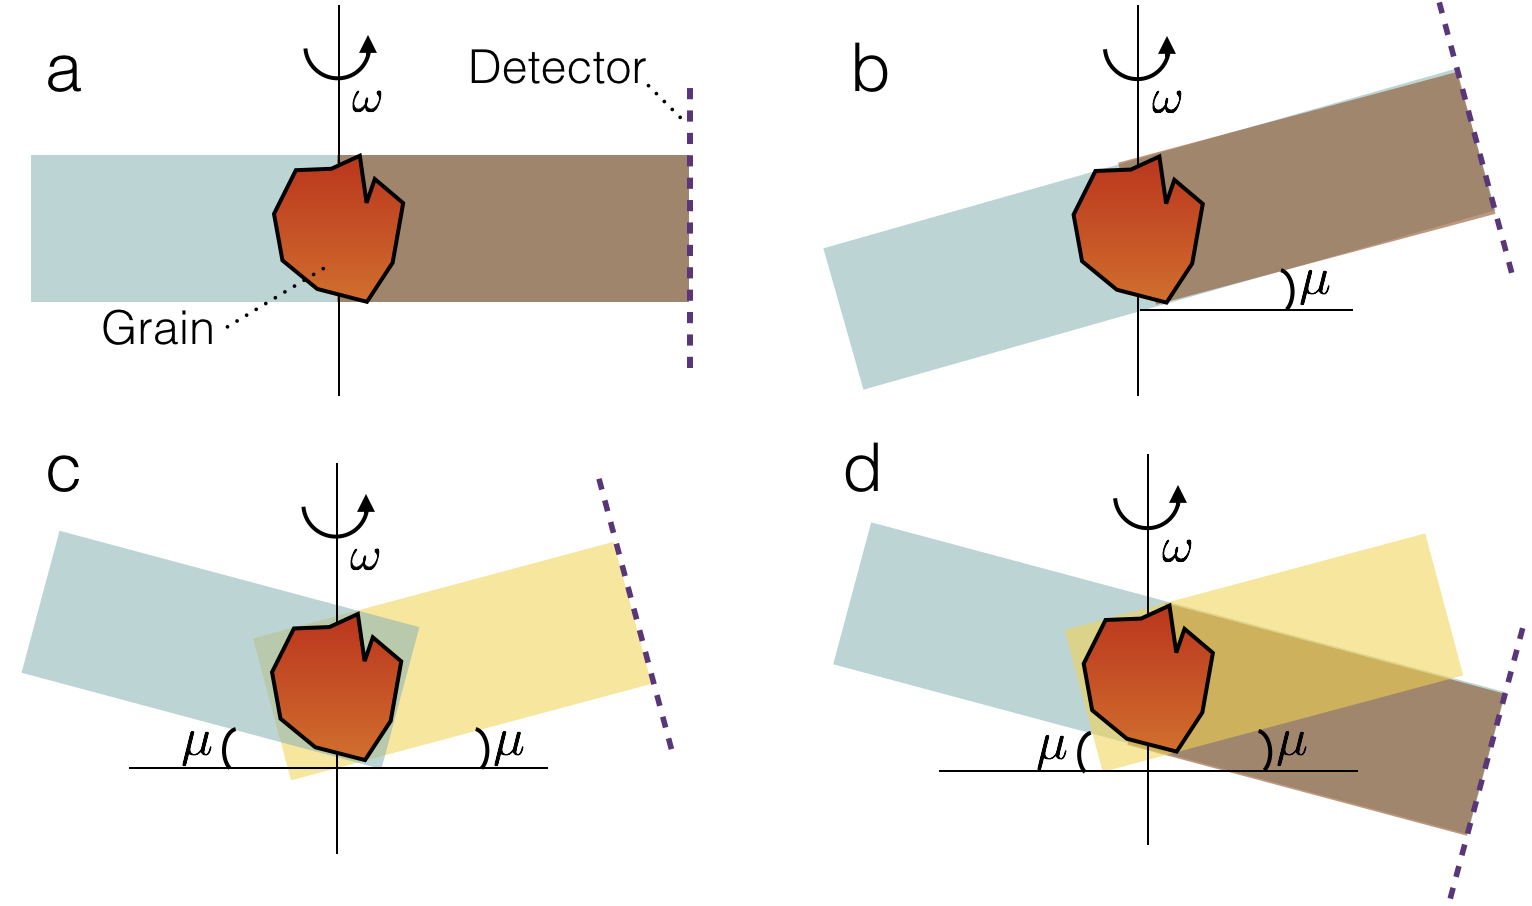
\includegraphics[width=0.75\textwidth]{ASTRA_recon3d_geom.png}
    \caption{The {\footnotesize{ASTRA}} toolbox is designed to reconstruct {\footnotesize{3D}} volumes from transmission data. To reconstruct a topotomo dataset collected using {\footnotesize{DFXRM}}, the diffraction data is considered instead. {\emph{a}}: standard {\footnotesize{CT}} geometry, with the incoming beam perpendicular to the sample rotation axis and to the {\footnotesize{2D}} detector collecting the transmitted signal. {\emph{b}}:  {\footnotesize{CT}} geometry with incoming beam inclined by $\mu$ with respect to the horizontal axis. {\emph{c}}: topotomography geometry. The incoming beam is inclined by $\mu$, and the diffracted beam by $\pi - \mu$. {\emph{d}}: with {\footnotesize{ASTRA}}, reconstructing a {\footnotesize{3D}} grain shape from data collected in diffraction at $\pi-\mu$ (setup in {\emph{c}}) corresponds to working with data collected in transmission at $\pi+\mu$.}
    \label{fig:astra_dfxrm}
\end{figure}

\subsubsection{Geometrical considerations}
\label{sec:astra_geom}

With the {\footnotesize{ASTRA}} toolbox, the {\footnotesize{DFXRM}} setup can be described using a parallel beam configuration. In this way, it is possible to ignore the source-to-rotation axis and the rotation axis-to-detector distances and use the {\texttt{parallel\textunderscore vec}} geometry. With {\texttt{parallel\textunderscore vec}}, the experimental geometry is described by four vectors: the ray direction ${\vec{r}}$, the detector center ${\vec{d}}$, and the two orthogonal detector vectors ${\vec{u}}$ and ${\vec{v}}$ (See Fig. \ref{fig:geom_setup}).

\begin{figure}[h]
    \centering
    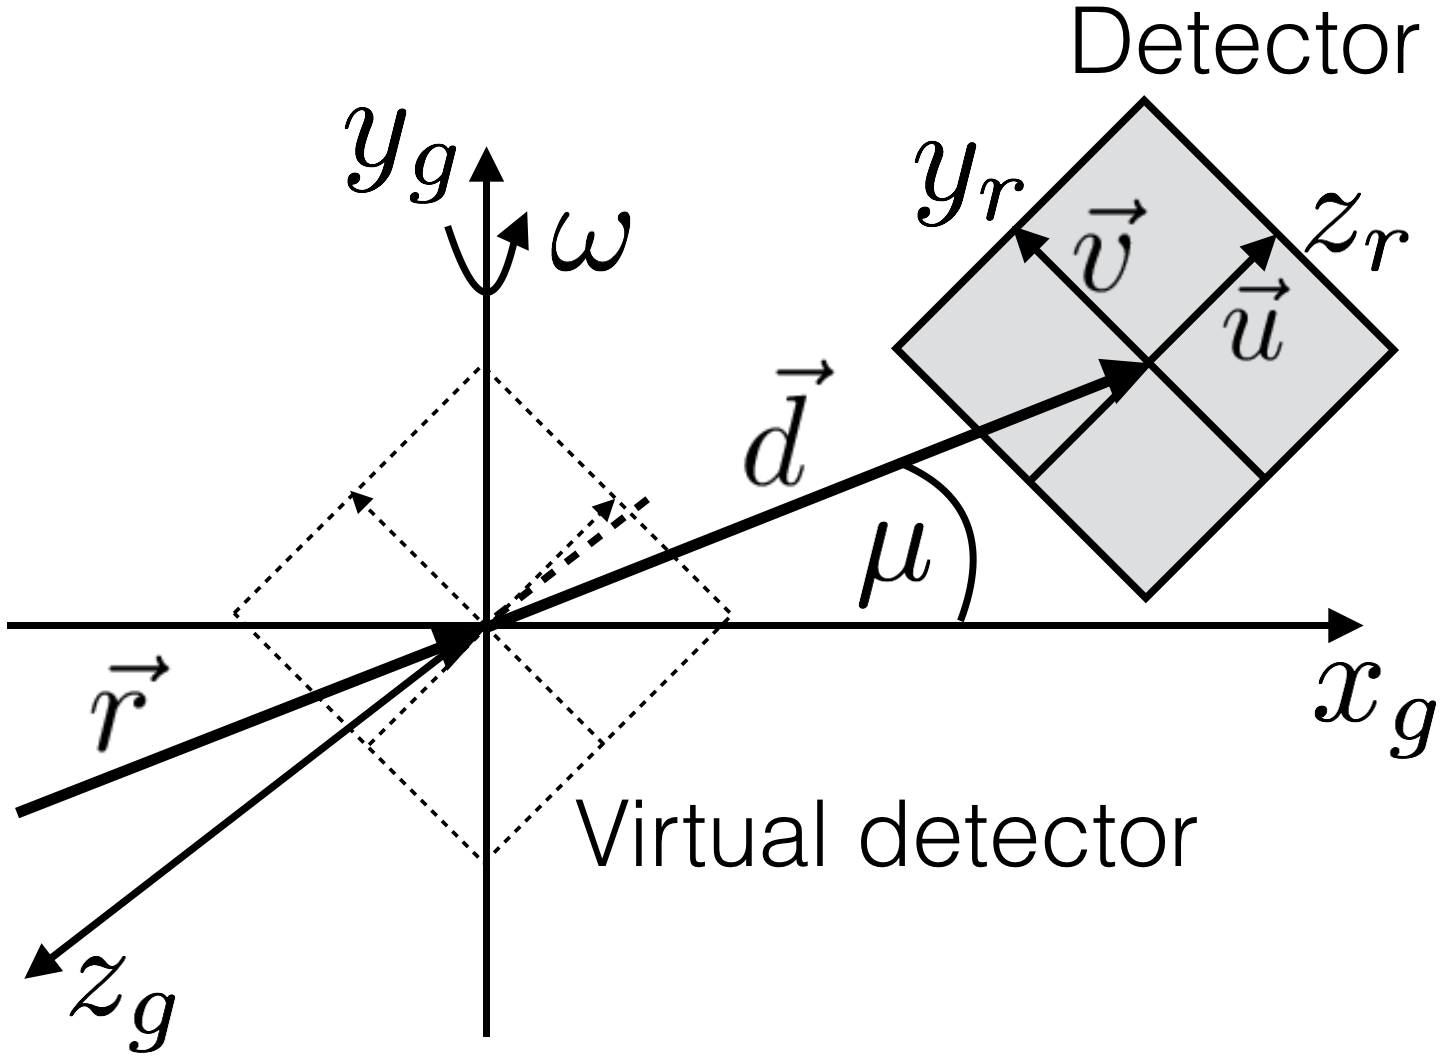
\includegraphics[width=0.4\textwidth]{geom_setup.png}
    \caption{Description of the topotomography setup using the {\footnotesize{ASTRA}} toolbox notation. $\omega$ is the sample rotation angle around the $y_g$ axis, $z_g$ is perpendicular (pointing towards the reader) to the $x_gy_g$-plane, $y_r$ and $z_r$ ($z_r \parallel z_g$, with $z_r$ pointing towards the reader) are the detector axes and $\mu$ is the angle formed by the incoming (and transmitted) beam with the horizontal axis. Following the {\texttt{parallel\textunderscore vec}} geometry, ${\vec{r}}$ is the incoming beam direction, ${\vec{d}}$ is the direction of the detector center, and ${\vec{u}}$ and ${\vec{v}}$ are the vectors defining the detector plane. The virtual detector is the detector translated along $\vec{r}$, so that the detector centre passes through the origin.}
    \label{fig:geom_setup}
\end{figure}

Using a ``virtual detector'' approach, the detector can be translated along the ray direction, so that the detector plane goes through the origin. In this way, all components of ${\vec{d}}$ can be set to zero, since the virtual detector now spins instead of moving around in a big circle.

To determine the components of ${\vec{r}}$, ${\vec{u}}$ and ${\vec{v}}$, let us first define the vectors at $\omega = 0$ (denoted as ${\vec{r_0}}$, ${\vec{u_0}}$, ${\vec{v_0}}$) and then calculate the more general case by rotating the vectors around $y_g$. ${\vec{r_0}}$ has no component in the $z_g$ direction and can be expressed as

\begin{equation}
{\vec{r_0}} = \left(\begin{matrix}
\cos\mu\\ \sin \mu\\ 0
\end{matrix}\right)
\end{equation}

${\vec{u_0}}$ should be along $z_r$, and have the same length of one detector pixel. Assuming that volume voxels have the same size of the detector pixels

\begin{equation}
{\vec{u_0}} = \left(\begin{matrix}
0\\ 0 \\ 1
\end{matrix}\right)
\end{equation}

\danger This needs to be changed if the detector size is different from the volume voxels size.

The third non-zero vector is ${\vec{v_0}}$

\begin{equation}
\vec{v_0} = \left(\begin{matrix}
-\sin\mu\\ \cos\mu\\ 0\\
\end{matrix}\right)
\end{equation}

At a given angle $\omega$, the components of ${\vec{r}}$, ${\vec{u}}$ and ${\vec{v}}$ can be calculated by rotating $\vec{r_0}$, $\vec{u_0}$ and $\vec{v_0}$ around the $y_g$ axis using a rotation matrix $R_y$. For counterclockwise rotations

\begin{equation}
R_y(\omega) = \begin{pmatrix}
\cos \omega & 0 & \sin \omega \\
0 & 1 & 0 \\
-\sin \omega & 0 & \cos \omega \\
\end{pmatrix}
\end{equation}

Which gives $\vec{r} = R \vec{r_0}$, $\vec{u} = R \vec{u_0}$ and $\vec{v} = R \vec{v_0}$.

\subsubsection{The ASTRA scripts}

The scripts developed to reconstruct a topotomography dataset using the {\footnotesize{ASTRA}} toolbox are available at \url{https://github.com/albusdemens/astrarecon}.

\danger The scripts are still under development.

The recipe to reconstruct a {\footnotesize{3D}} grain shape is:
\begin{enumerate}
    \item For each projection, sum all collected images using {\texttt{getdata.py}}. As input, the script takes the numpy arrays returned by {\texttt{getdata.py}}, part of the Recon3D package (Sec. \ref{script:getdata}, details in Sec. \ref{sec:getdata}). Both scripts run on Panda2.
    \begin{itemize}
        \item Command: {\texttt{\$ python getdata.py [Input directory] [Modality]}} \newline  {\texttt{[Lower threshold] [Upper threshold]}}. {\texttt{Input directory}} is the output directory of {\texttt{getdata.py}} (part of Recon3D); {\texttt{Modality}} is 1 to determine threshold and rotation centre, 2 to determine rotation axis and 3 to prepare data for reconstruction; {\texttt{Lower threshold}} and {\texttt{Upper threshold}} are, respectively, the lower and upper threshold values used to clean the summed images
        \item Usage: first run the script in modality 1 to determine the possible threshold values, then run in modality 3
        \item Output: Sum, projection by projection, of the collected frames. Data are stored both as {\texttt{.npy}} (for Python) and as {\texttt{.mat}} (for {\footnotesize{MATLAB}})
    \end{itemize}
    \item Reconstruct the {\footnotesize{3D}} shape of the considered grain using {\texttt{recon.py}}. In the current version, the grain shape is reconstructed using the {\footnotesize{SIRT}} algorithm. The code is designed to run on a {\footnotesize{GPU}}-equipped machine
    \begin{itemize}
        \item Command: {\texttt{\$ python recon.py [Input folder]}}. {\texttt{Input folder}} is the directory with the summed images returned by {\texttt{getdata.py}} (previous step)
        \item Output: set of {\texttt{.png}} files. Each image is a layer of the reconstructed volume
    \end{itemize}
    \item Check the reconstruction quality using {\texttt{makemovie.py}}. The script runs on a {\footnotesize{GPU}} machine; to visualize the results copy the output to your machine or to Panda2
\end{enumerate}

\subsection{Validation using ART-TV}

At present (November 2017) the best grain shape reconstructions have been obtained using the {\footnotesize{ART-TV}} approach. The starting point to define the {\footnotesize{ART-TV}} geometry is the reconstruction geometry used with the {\footnotesize{ASTRA}} toolbox (Sec. \ref{sec:astra_geom}) where, instead of the diffraction signal, the corresponding transmission signal is considered.

The available version of the {\footnotesize{ART-TV}} algorithm only works with an incoming beam that is perpendicular to the sample rotation axis and to the detector. By reconstructing, instead of the considered sample, an approximation of it, {\footnotesize{ART-TV}} can also be applied when the incoming beam is inclined by $\mu$ with respect to the horizontal axis.

\subsubsection{Geometrical considerations}

\begin{figure}
    \centering
    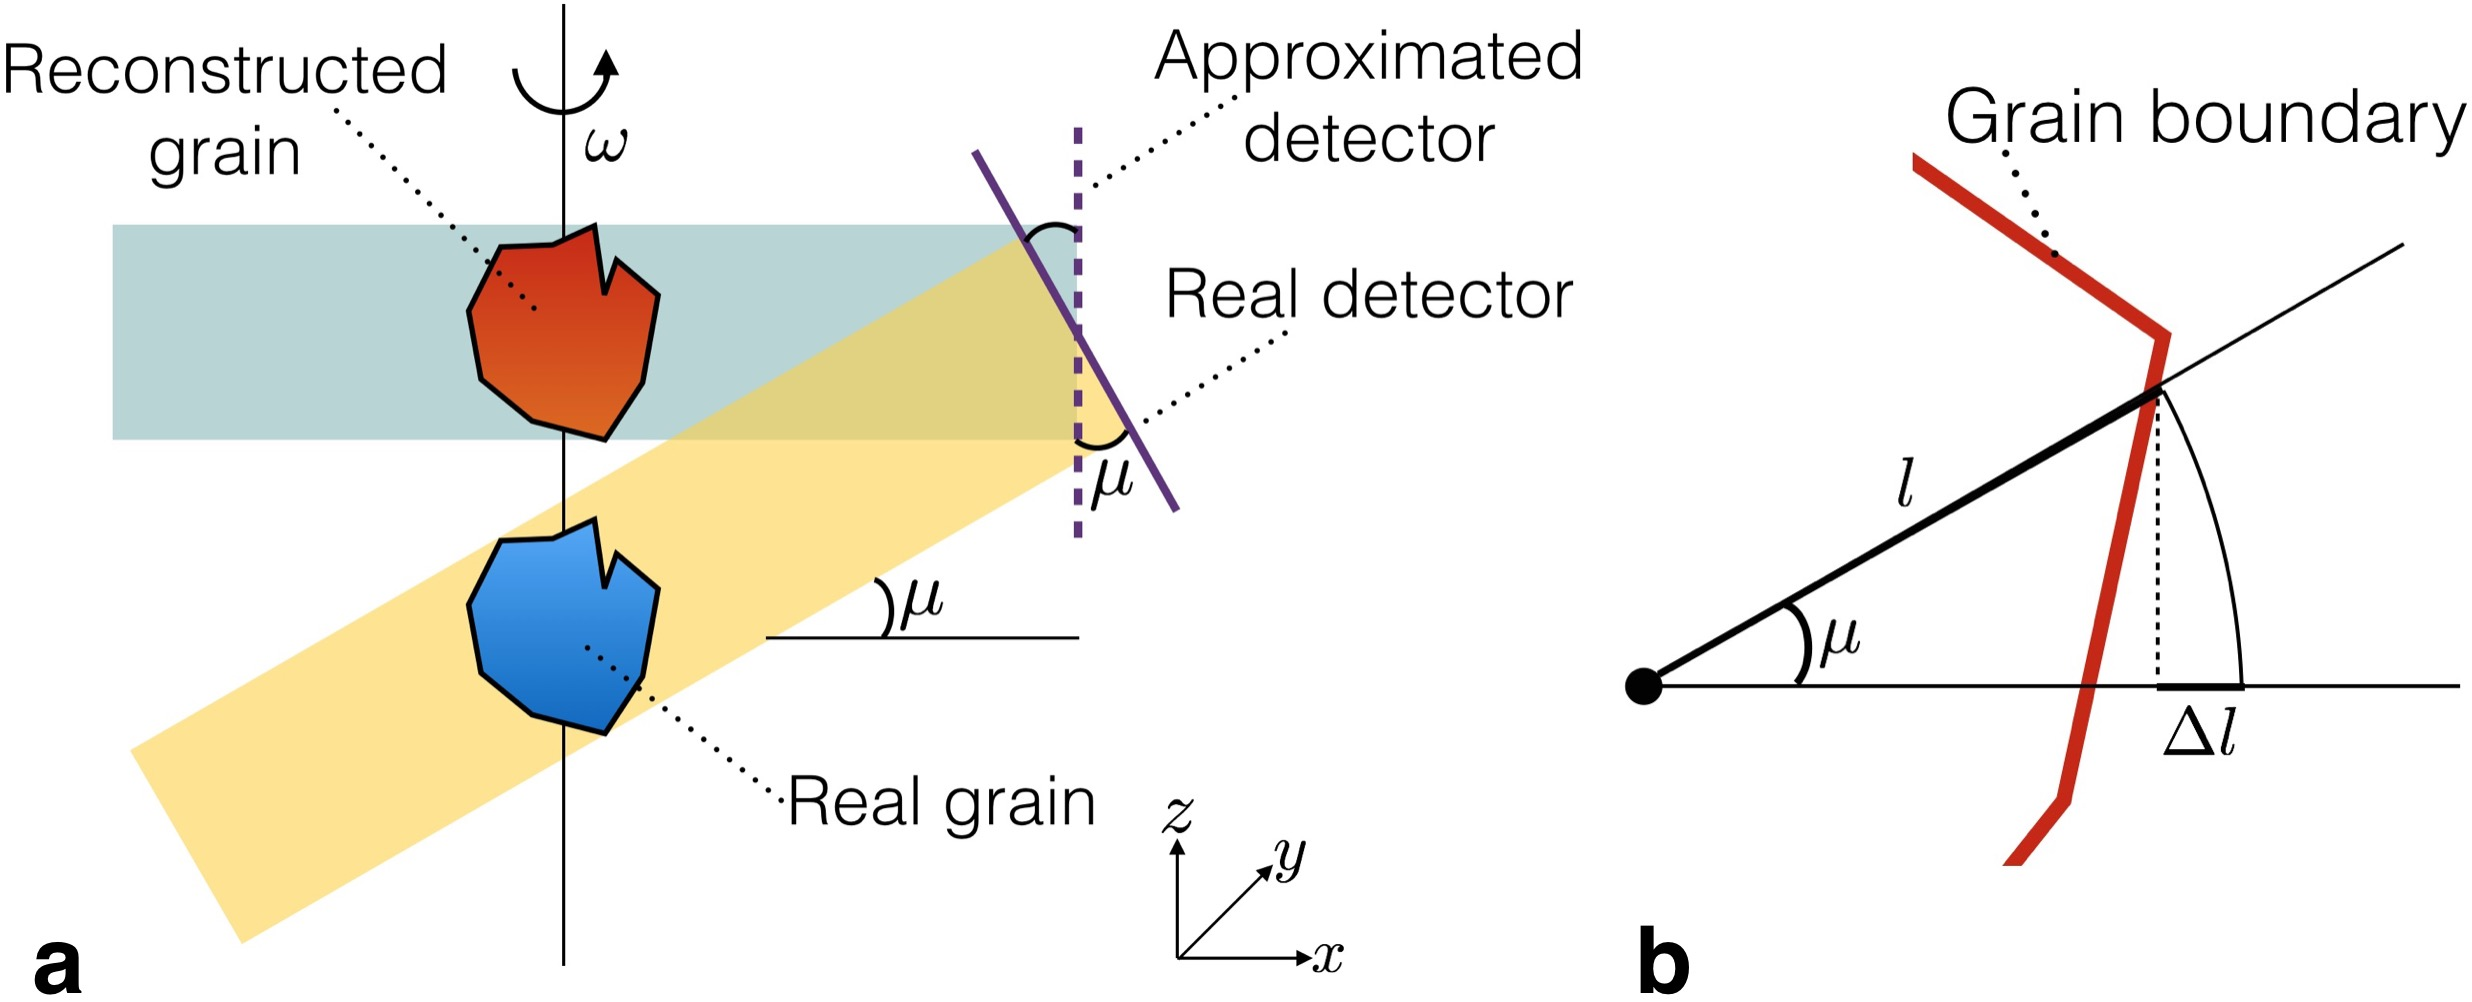
\includegraphics[width=0.8\textwidth]{geom_art_tv.png}
    \caption{Basic principle used to apply {\footnotesize{ART-TV}} to reconstruct the {\footnotesize{3D}} shape of a grain investigated using topotomography. In short, instead of the real sample an approximation of it is reconstructed. {\emph{(a)}}: Sketch of the transmission tomography geometry (real grain, real detector, beam inclined by $\mu$), and geometry used by the {\footnotesize{ART-TV}} technique ({\footnotesize{CT}} scan-like): the grain is reconstructed by considering the data as collected by the approximated detector. {\emph{(b)}}: a photon travelling from a voxel to the grain boundary along a path inclined by an angle $\mu$ covers a longer distance than a photon traveling along an horizontal line with the same exit point. Covering a longer distance, information about more voxels is collected. As a consequence, the reconstructed grain is expected to be about $\Delta l = 1-\cos\mu$ wider (on the horizontal plane) than the real grain. In first approximation, the grain height remains constant.}
    \label{fig:art_tv_geometry}
\end{figure}

The applied {\footnotesize{ART-TV}} code is designed to reconstruct {\footnotesize{3D}} shapes collected in standard parallel beam geometry, with the beam perpendicular to both the rotation axis and the detector plane. Therefore, applying {\footnotesize{ART-TV}} to the topotomo data returns an approximation of the ``real'' shape. The reconstructed shape can be estimated to be $\sim 1 - cos\theta$ wider, in the {\footnotesize{XY}} plane, than the real shape, as illustrated in Fig \ref{fig:art_tv_geometry}.

To derive this estimate, let us consider a photon travelling from a voxel to the grain boundary. In the real configuration, the photon path is inclined by an angle $\mu$ with respect to the horizontal axis and has length {\emph{l}}, $\Delta l$ longer that the path covered by a photon flying parallel to the {\footnotesize{X}} axis, with the same grain boundary exit point. Therefore, a rough estimate of the grain deformation due to the improper geometry definition is that the reconstructed grain is about $\Delta l$ larger on the {\footnotesize{XY}} plane than the real grain.

In formulas,

\begin{eqnarray}
    l - \Delta l & = & l\cdot\cos\theta \\
    \Delta l & = & l (1 - \cos\theta)
\end{eqnarray}

For $\theta = 10.38^{\circ}$, this corresponds to an horizontal dilation of about $ 1 - \cos(10.38^{\circ}) = 1 - 0.984 = 1.6 \%$. We consider the height of the reconstructed grain to be consistent with the height of the real grain. Before comparing, at a given angle, the projection of the reconstructed volume with the sum of the collected diffraction signal, the projection was eroded to take into account possible horizontal dilations.

\subsubsection{The ART-TV scripts}

The scripts developed to reconstruct a topotomography dataset using {\footnotesize{ART-TV}} are available at \url{https://github.com/albusdemens/ART-TV-for-DFXRM}.

\begin{figure}[h]
    \centering
    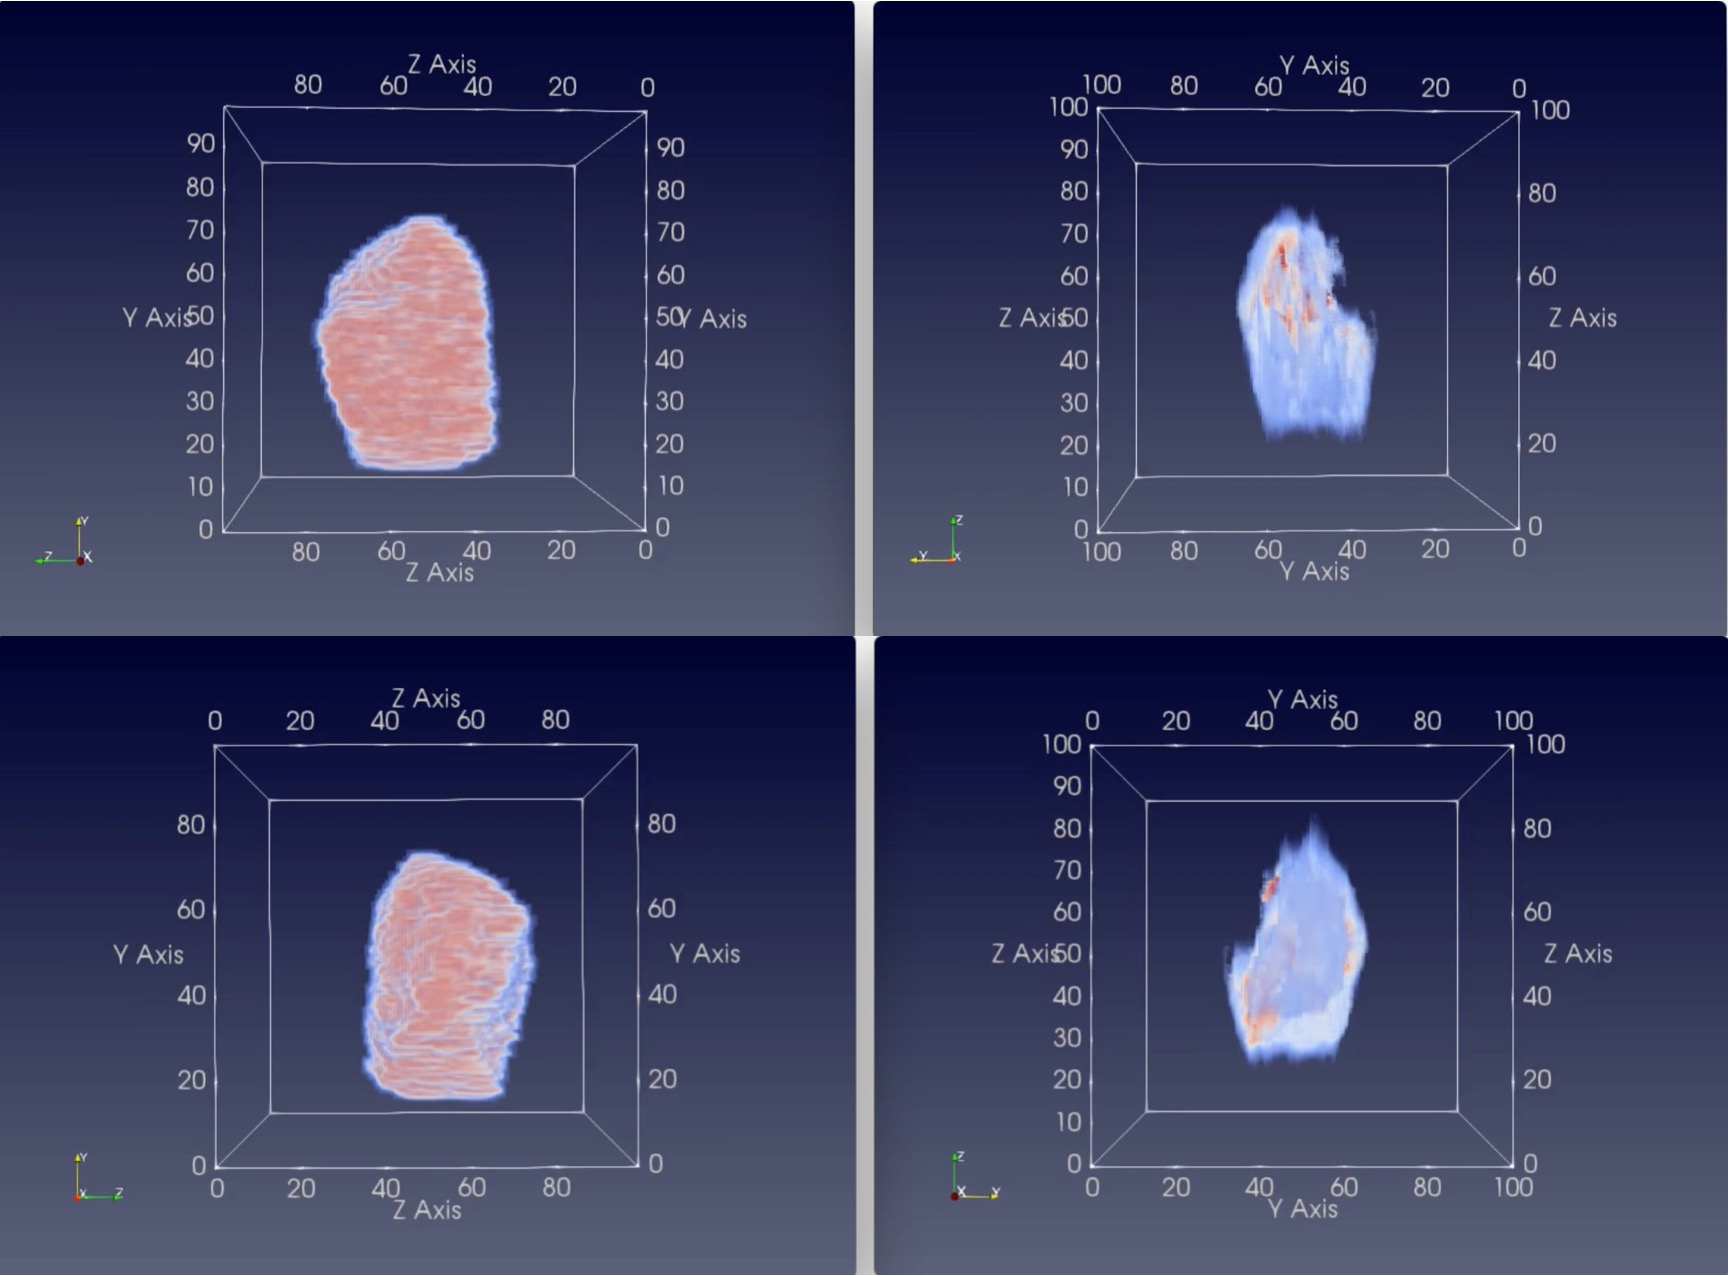
\includegraphics[width=0.8\textwidth]{Comparison_ART_recon3d.png}
    \caption{Comparison of the 3D grain shape reconstructed using {\footnotesize{ART-TV}} ({\emph{left}}) and using Recon3D ({\emph{right}}). Sample: Al grain, imaged at {\footnotesize{ID06}}}
    \label{fig:vol_ART_recon3d}
\end{figure}

Using {\footnotesize{ART-TV}}, the recipe to reconstruct the grain shape is:
\begin{enumerate}
    \item Sum, projection by projection, all collected images, using the scripts {\texttt{getdata.py}} and {\texttt{img\textunderscore sum.py}}, included in Recon3D
    \item Reconstruct the sample using {\texttt{reconstr.m}}. The script takes as input the {\texttt{.mat}} file returned by {\texttt{img\textunderscore sum.py}}. For a comparison of the {\footnotesize{3D}} grain shape reconstructed using Recon3D and {\footnotesize{ART-TV}}, see Fig. \ref{fig:vol_ART_recon3d}
    \item Compare the volume reconstructed using {\footnotesize{ART-TV}} with the reconstruction returned by Recon3D and with the experimental data (see Fig. \ref{fig:compare_proj}). Script: {\texttt{Compare\textunderscore recon3d\textunderscore ART.m}}. The script also combines information from the Recon3D reconstruction and from the {\footnotesize{ART-TV}} one in a single volume: the shape of the volume is defined by {\texttt{ART-TV}}, and the voxels in the volume have the orientation returned by Recon3D.

    Use the {\texttt{deadTHreshparameter}} to exclude certain projections from the reconstruction. Usually, the reconstruction quality increases with the numb er of available projections.
\end{enumerate}

Inside the volume reconstructed combining {\footnotesize{ART-TV}} and Recon3D, the voxels have orientation defined by the $\gamma, \mu$ values assigned using Recon3D.

For the selected volume, the grain orientation can be represented by rescaling the $\gamma$ and $\mu$ values to the $[0,1]$ interval, and then calculating the corresponding HSV color:

\begin{verbatim}

h(i) = wrapTo2Pi(atan2(vr,ur))/pi/2;

s(i) = sqrt(ur^2+vr^2)/sqrt(2);

v(i) = 1;

\end{verbatim}

Where {\texttt{ur}} and {\texttt{vr}} are $\mu$ and $\gamma$, respectively.

By plotting the {\footnotesize{Z}} slices of the grain volume, subgrain structures can be observed (see Fig. \ref{fig:mosaicity_slice}).

\begin{figure}
    \centering
    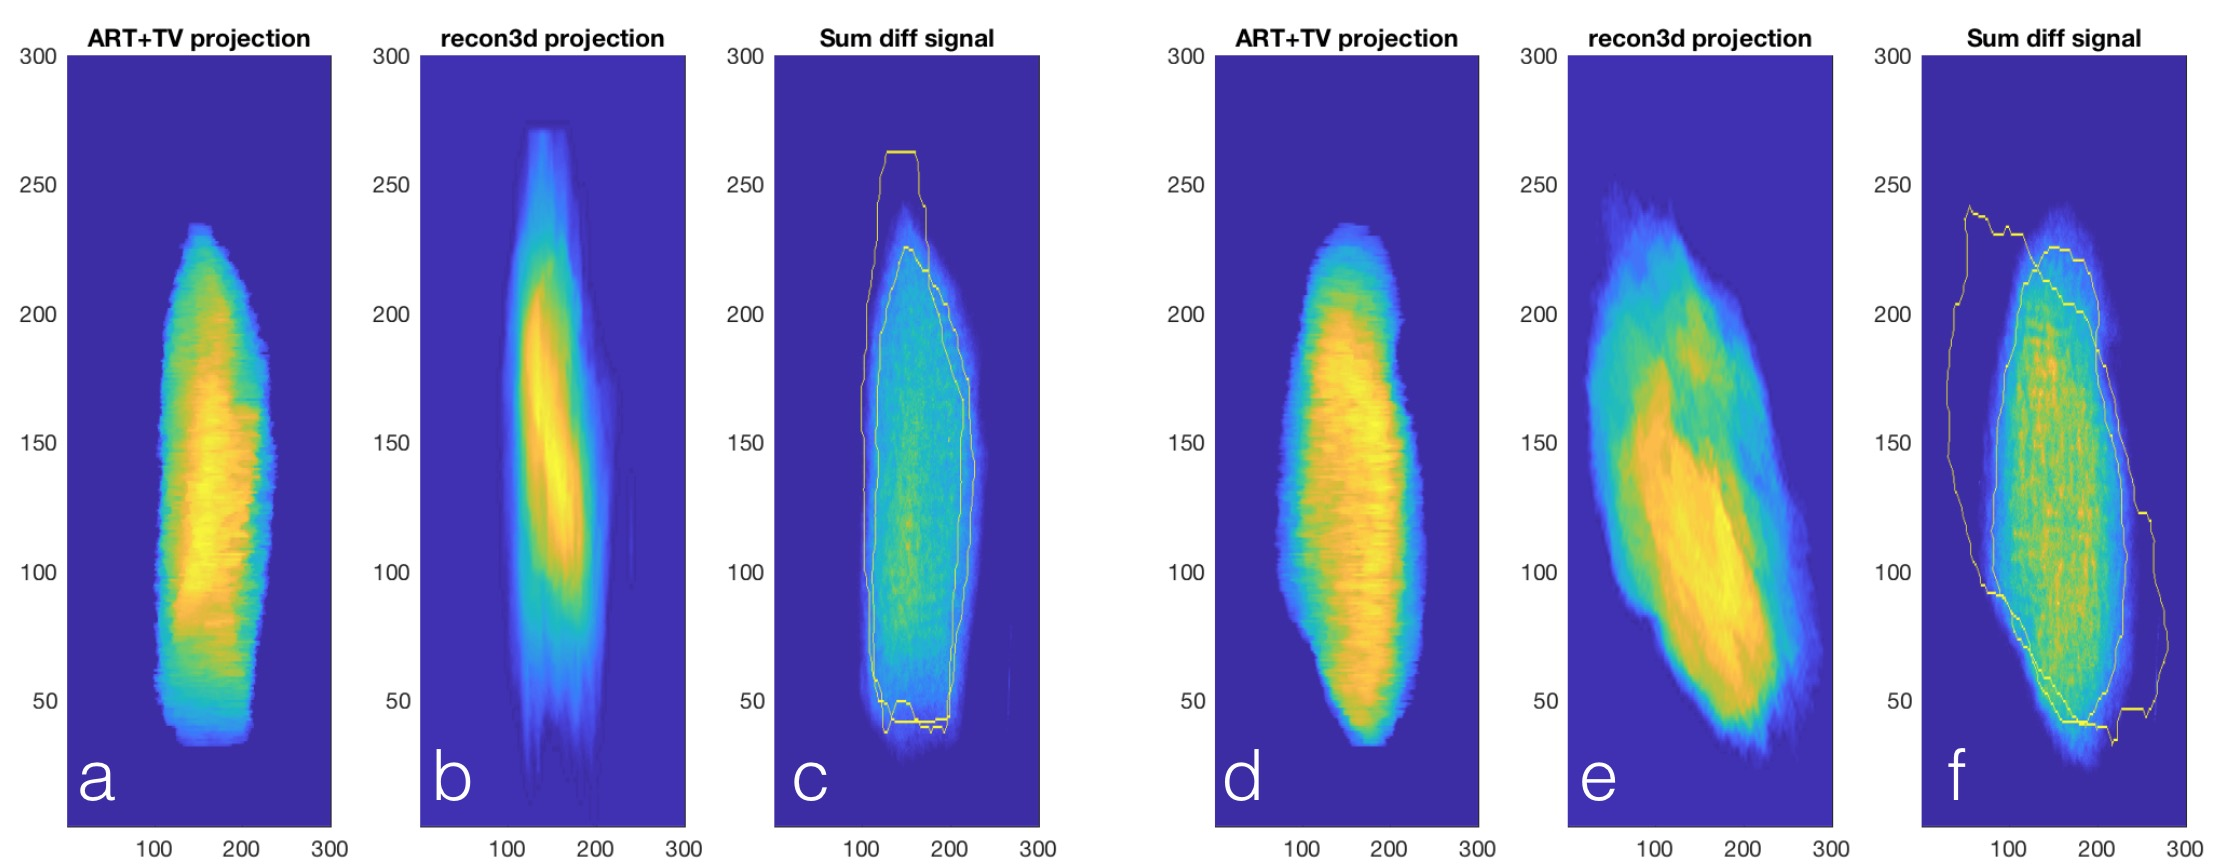
\includegraphics[width=0.95\textwidth]{compare_proj_diff_all_proj.png}
    \caption{To validate the 3D reconstructions returned by {\footnotesize{ART-TV}} and Recon3D, the corresponding volumes were projected and compared with the sum of the diffraction data recorded at the corresponding rotation angle. Here for two rotation angles the projection of the {\footnotesize{3D}} reconstruction obtained using {\footnotesize{ART-TV}} ({\emph{a}} and {\emph{d}}) is compared with the projection of the Recon3D reconstruction ({\emph{b}} and {\emph{e}}) and with the sum of the diffraction data ({\emph{c}} and {\emph{f}}). In {\emph{c}} and {\emph{f}}, the eroded profile of the projected volumes is shown as a yellow line. Data relative to an Al grain investigated at {\footnotesize{ID06}}.}
    \label{fig:compare_proj}
\end{figure}

\begin{figure}[h]
    \centering
    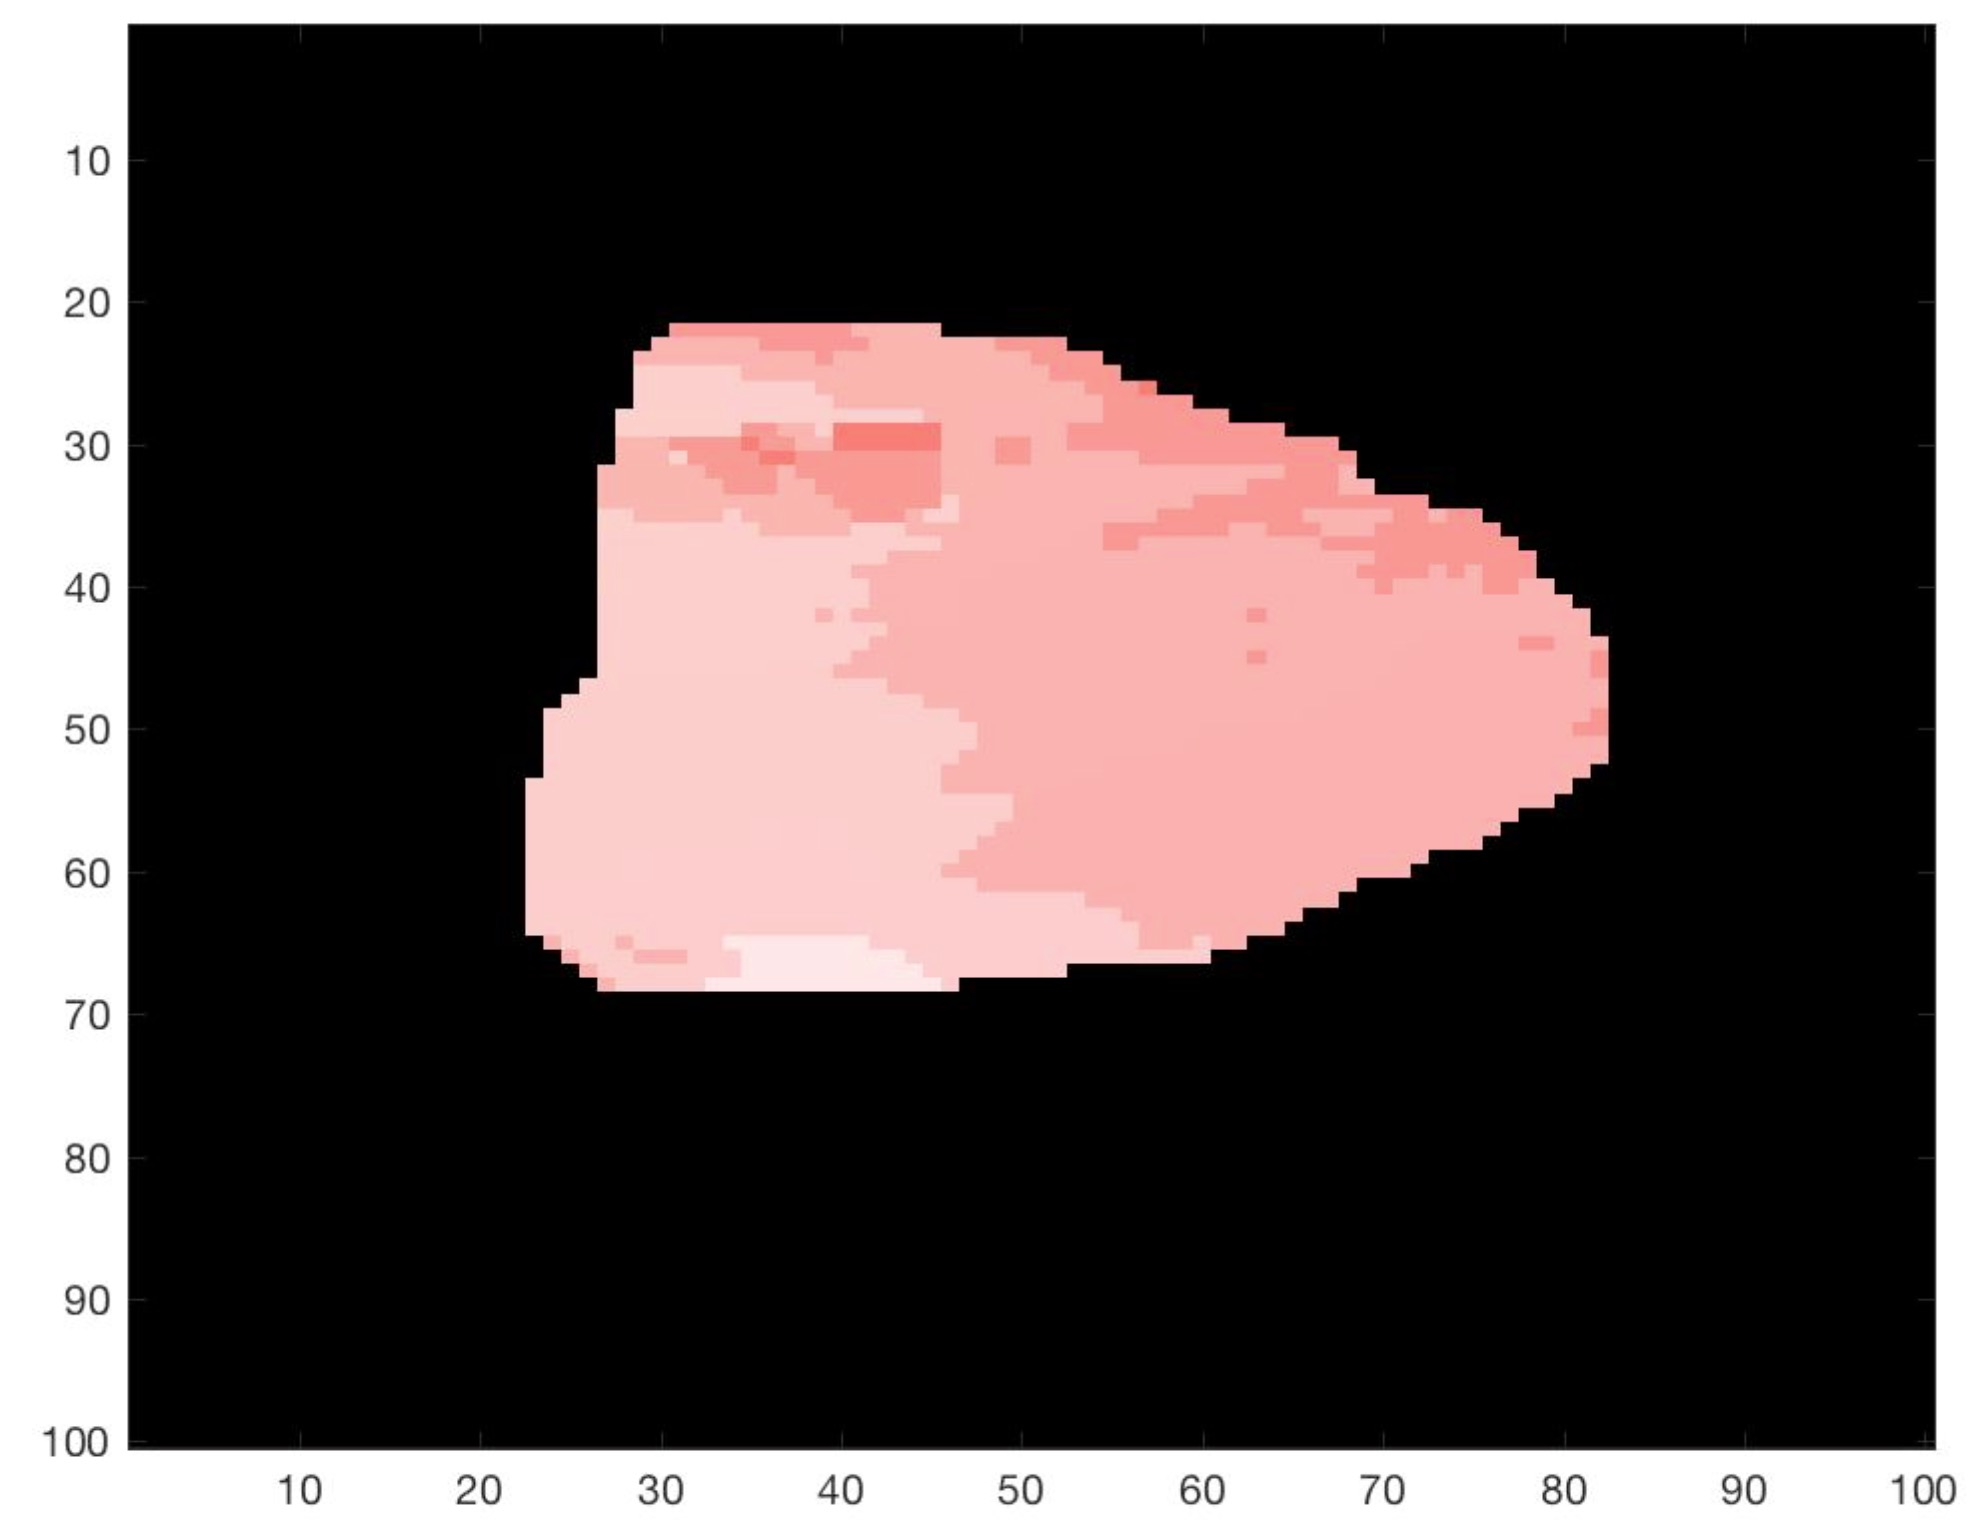
\includegraphics[width=0.65\textwidth]{Mosaicity_slice_new.png}
    \caption{Slice of the reconstructed grain volume, with different subgrains shown in different colors. The {\footnotesize{HSV}} representation is used. Data relative to an Al grain investigated at {\footnotesize{ID06}}.}
    \label{fig:mosaicity_slice}
\end{figure}

\section{To dos}

\subsection{Critical}

\begin{enumerate}
    \item In {\texttt{getdata.py}}, include the option to consider the case when the diffraction signal covers the entire frame, and the cornice method cannot be used
    \item Determine if, to find which ($\gamma, \mu$) describes the orientation of a voxel, it is {\footnotesize{OK}} to consider the location of the max in the summed mosaicity map. What if we have two max? Idea: combine max, {\footnotesize{CM}}
\end{enumerate}

\subsection{Will make life easier}

\begin{enumerate}
    \item Provide paths as input in
    \begin{itemize}
        \item {\texttt{rebin\textunderscore img.py}}
        \item {\texttt{plot\textunderscore img.py}}
        \item {\texttt{plot\textunderscore angles.py}}
    \end{itemize}
    \item Install ImageJ and/or {\footnotesize{FIJI}} on Panda2, to visualize stack of images without the need to download them
    \item Install ParaView on Panda2, to visualize {\footnotesize{3D}} vtk files
    \item Combine {\texttt{img\textunderscore sum.py}} and {\texttt{plot\textunderscore sum.py}}
    \item {\texttt{plot\textunderscore angles.py}} should also return a sinogram of the collected data
    \item Some of the data analysis programs are in Matlab. Having them in Pyhton instead would unify the code and make it easier to script programs
\end{enumerate}

\subsection{Would be nice to have}

\begin{enumerate}
    \item Adapted version of {\texttt{fabian}} (included in FabIO \cite{knudsen2013fabio}) for visualizing sets of {\texttt{.edf}} files. At the moment, {\texttt{fabian}} only works for list of files numbered incrementally. Usually, the images collected during a topotomo scan are named {\texttt{file\textunderscore XXX\textunderscore YYY.edf}}, with {\texttt{YYY}} going from 0 to the number of angular steps (one motor only), and {\texttt{XXX}} increasing by 1 after {\texttt{YYY}} went through all motor values
\end{enumerate}

\section{Code contributors}

In alphabetic order:
\begin{itemize}
    \item Alberto Cereser, contributor 2017

    Email: \href{alberto.cereser@gmail.com}{alberto.cereser@gmail.com}, \href{alcer@fysik.dtu.dk}{alcer@fysik.dtu.dk}

    Recon3D repository: \href{https://github.com/albusdemens/Recon3D}{https://github.com/albusdemens/Recon3D}

    \item Anders Clemen Jakobsen, contributor 2016/2017

    Email: \href{andcj@fysik.dtu.dk}{andcj@fysik.dtu.dk}

    Recon3D repository: \href{https://github.com/acjak/Recon3D}{https://github.com/acjak/Recon3D}

\end{itemize}

\bibliographystyle{ieeetr}
\bibliography{Manual_DFXRM_software}

\end{document}
